\chapter{Αντιστοίχιση με Αλγορίθμους Μετανοητικής Μάθησης}

Σε αυτό το κεφάλαιο της διπλωματικής εργασίας θα μελετήσουμε έναν αλγόριθμο Μετανοητικής Μάθησης και θα τον συγκρίνουμε με τον αλγόριθμο Θεωρίας Παιγνίων που αναπτύξαμε στο κεφάλαιο 2. Η Μετανοητική Μάθηση (Regret Learning) είναι μια έννοια που βασίζεται στη θεωρία παιγνίων και τη μηχανική μάθηση, ιδιαίτερα σημαντική στο πλαίσιο των επαναλαμβανόμενων παιγνίων και της ενεργής μάθησης. Εστιάζει στην ελαχιστοποίηση της ενοχής (μετάνοια), ορισμένης ως η διαφορά μεταξύ της απόδοσης μιας στρατηγικής λήψης αποφάσεων και της βέλτιστης στρατηγικής με βάση την αναδρομική θεώρηση, σε επαναλαμβανόμενες αλληλεπιδράσεις ή επαναλήψεις. \lcite{regretchapter}

Υπάρχουν δύο κύριοι τύποι ενοχής: η εξωτερική ενοχή, η οποία μετράει πόσο χειρότερα απέδωσε μια στρατηγική σε σύγκριση με την καλύτερη σταθερή δράση με βάση την αναδρομική θεώρηση, και η εσωτερική ενοχή, η οποία συγκρίνει την απόδοση με την καλύτερη προσαρμοστική πολιτική, όπου ο παίκτης θα μπορούσε να αλλάξει δράσεις με βάση τα προηγούμενα αποτελέσματα. Αλγόριθμοι ελαχιστοποίησης της ενοχής σχεδιάζονται για να ενημερώνουν τις πιθανότητες των δράσεων με βάση τις προηγούμενες αποδόσεις, ώστε να ελαχιστοποιήσουν την ενοχή. Αυτοί οι αλγόριθμοι έχουν εφαρμογές σε διάφορους τομείς. Για παράδειγμα στην ενεργή μάθηση, όπου βοηθούν τους αλγορίθμους να μαθαίνουν από διαδοχικά δεδομένα σε αντίπαλα περιβάλλοντα. Επιπλέον στη θεωρία παιγνίων, ιδιαίτερα σε επαναλαμβανόμενα παίγνια όπου οι παίκτες προσαρμόζουν τις στρατηγικές τους με βάση τα προηγούμενα αποτελέσματα, και στη μάθηση με ενίσχυση, όπου οι παίκτες μαθαίνουν πολιτικές για τη μεγιστοποίηση των ανταμοιβών με την πάροδο του χρόνου. \lcite{regretchapter}

Τα οφέλη της Μετανοητικής Μάθησης περιλαμβάνουν την προσαρμοστικότητα, καθώς οι αλγόριθμοι μπορούν να προσαρμοστούν σε μεταβαλλόμενα περιβάλλοντα και να αποδώσουν καλά υπό διάφορες συνθήκες, και τη στιβαρότητα, που τους επιτρέπει να αντιμετωπίζουν ανταγωνιστικές καταστάσεις όπου οι αντίπαλοι μπορεί να προσπαθήσουν να εκμεταλλευτούν αδυναμίες (\lcite{Xu2024}, \lcite{Abramson2015}). Τα θεωρητικά θεμέλια της ελαχιστοποίησης της ενοχής περιλαμβάνουν τη θεωρία πιθανοτήτων, την κυρτή ανάλυση και τη βελτιστοποίηση, με βασικά αποτελέσματα που συχνά παρέχουν όρια στην ενοχή που μπορεί να επιτευχθεί από συγκεκριμένους αλγόριθμους. Συνολικά, η μάθηση με βάση την ενοχή προσφέρει ένα στιβαρό πλαίσιο για τη λήψη αποφάσεων σε αβέβαια και ανταγωνιστικά περιβάλλοντα, διασφαλίζοντας ότι οι στρατηγικές αποδίδουν βέλτιστα με την πάροδο του χρόνου, ελαχιστοποιώντας το χάσμα μεταξύ της πραγματικής και της ιδανικής απόδοσης.

Μέχρι τώρα μελετούσαμε το πως θα πρέπει να κατανεμηθούν οι κόμβοι στους εξυπηρετητές για να επιτύχουμε το καλύτερο δυνατό αποτέλεσμα στην Ομοσπονδιακή Μάθηση. Στο κομμάτι που ακολουθεί, αυξάνουμε το χώρο ενεργειών του κάθε κόμβου, δηλαδή του επιτρέπουμε να αλλάξει τιμές στα βασικά του μεγέθη επιλέγοντας πόσους πόρους θα θέλει ο ίδιος να διαθέσει για την Ομοσπονδιακή Μάθηση. Παρακάτω θα δούμε και πιο αναλυτικά τις παραμέτρους τις οποίες ο κάθε κόμβος μπορεί να μεταβάλλει για το συμφέρον του. Πολυδιάστατα, σαν αυτό, προβλήματα αυξάνουν πολύ σε πολυπλοκότητα όσο αυξάνεται και ο χώρος καταστάσεων που μπορούμε να έχουμε. Όμως, μπορούν να μας δώσουν και μεγάλα κέρδη σε χρησιμότητα, αφού εκ' φύσεως ο κάθε κόμβος έχει διαφορετικές βλέψεις και συμφέροντα σε ένα περιβάλλον Ομοσπονδιακής Μάθησης.

\section{Περιγραφή Αλγορίθμου Μετανοητικής Μάθησης}

Όπως αναφέραμε, πλέον κάθε κόμβος μπορεί να ελέγχει σε μεγαλύτερο βαθμό την συμπεριφορά του εντός του οικοσυστήματος. Συγκεκριμένα, μπορεί να προσαρμόζει τους διαθέσιμους πόρους του για να μεγιστοποιήσει το όφελος του, δηλαδή να αλλάξει την ισχύ μετάδοσης $P_{n,s}$, την συχνότητα του ρολογιού της ΚΜΕ του $f_n$ και το μέγεθος του συνόλου δεδομένων που θα διαθέσει στην μάθηση $D_n$.

Για να μοντελοποιήσουμε πιο ρεαλιστικά το οικοσύστημά μας, αλλάζουμε λίγο τα εμπλεκόμενα μεγέθη που είδαμε στο κεφάλαιο 2. Έτσι, αντί για ποιότητα δεδομένων $d_n$, ενσωματώνουμε την παράμετρο $D_n$ στην πληρωμή που λαμβάνει ένας κόμβος από τον εξυπηρετητή. Δηλαδή όσο περισσότερα δεδομένα προσφέρει ένας κόμβος στον εξυπηρετητή του, τόσο καλύτερες απολαβές θα έχει. Αντίστοιχα, ενσωματώνουμε και την παράμετρο $f_n$ στην πληρωμή από τον εξυπηρετητή. Επιπλέον, κάθε κόμβος λαμβάνει απολαβές από τον εξυπηρετητή ανάλογα με τη σημασία του, αφού ένας εξυπηρετητής δεν θα ήθελε να πληρώνει το ίδιο έναν σημαντικό και έναν όχι τόσο σημαντικό κόμβο. Οπότε, με βάση τις παραπάνω παρατηρήσεις, διαμορφώνουμε την κανονικοποιημένη πληρωμή του κόμβου από τον εξυπηρετητή ως:

\vspace{-5pt}

\begin{equation}
\hat{Pnt}_{n,s}=\frac{c_{n,s}\times current\_fn*ud_n}{max\_f_n\times max\_d_n}
\label{eq20}
\end{equation}

\vspace{-3pt}

\noindent
όπου $c_{n,s}$ η σημασία δεδομένων του κόμβου, $current\_fn$ η τιμή της συχνότητας της ΚΜΕ που επιλέγει ο κόμβος να χρησιμοποιήσει, $ud_n$ το μέγεθος του συνόλου δεδομένου που επιλέγει ο κόμβος να διαθέσει, $max\_f_n$ η μέγιστη συχνότητα της ΚΜΕ του κόμβου και $max\_d_n$ το μέγιστο σύνολο δεδομένων που διαθέτει ο κόμβος.

Αντίστοιχα για τα υπόλοιπα μεγέθη που μελετήσαμε, τα κανονικοποιούμε με τον ίδιο τρόπο και έχουμε τις παρακάτω εξισώσεις:

\vspace{-5pt}

\begin{equation}
\hat{R}_{n,s} = \frac{R_{n,s}}{Rmax_{n,s}}
\label{eq21}
\end{equation}

\vspace{-3pt}

\[R_{n,s} = B \log_2(1 + \frac{g_{n,s}\times current\_P_{n,s}}{\sum \limits_{n'\in s, n'\neq n} g_{n',s}P_{n',s} + g_{n,s}\times current\_P_{n,s} + I_0}) \quad [bps]\]

\[Rmax_{n,s} = B \log_2(1 + \frac{g_{n,s}\times max\_P_{n,s}}{\sum \limits_{n'\in s, n'\neq n} g_{n',s}P_{n',s} + g_{n,s}\times max\_P_{n,s} + I_0}) \quad [bps]\]

\noindent
όπου $current\_P_{n,s}$ δηλώνει την ισχύ μετάδοσης που επιλέγει ο κόμβος, $max\_P_{n,s}$ είναι η μέγιστη ισχύ μετάδοσης που μπορεί να διαθέσει ο κόμβος και άρα $R_{n,s}$ είναι ο ρυθμός μετάδοσης που πετυχαίνει ο κόμβος και $Rmax_{n,s}$ είναι ο μέγιστος ρυθμός μετάδοσης που μπορεί να πετύχει ο κόμβος με βάση την τωρινή κατάσταση του συστήματος.

\vspace{-5pt}

\begin{equation}
\hat{E}_n=\frac{\frac{a_n}{2}q_n\times ud_n\times current\_f_n^2}{\frac{a_n}{2}q_n\times max\_d_n\times max\_f_n^2} = \frac{ud_n\times current\_f_n^2}{max\_d_n\times max\_f_n^2}
\label{eq22}
\end{equation}

\vspace{-3pt}

\noindent
όπου $current\_f_n$ η τιμή της συχνότητας της ΚΜΕ που επιλέγει ο κόμβος να χρησιμοποιήσει, $ud_n$ το μέγεθος του συνόλου δεδομένου που επιλέγει ο κόμβος να διαθέσει, $max\_f_n$ η μέγιστη συχνότητα της ΚΜΕ του κόμβου και $max\_d_n$ το μέγιστο σύνολο δεδομένων που διαθέτει ο κόμβος.

\vspace{-5pt}

\begin{equation}
\hat{E}_{n,s}=\frac{\frac{Z(\mathbf{w}n)\times current\_P{n,s}}{R_{n,s}}}{\frac{Z(\mathbf{w}n)\times max\_P_{n,s}}{Rmax_{n,s}}} = \frac{current\_P_{n,s}\times Rmax_{n,s}}{max\_P_{n,s}\times R_{n,s}}
\label{eq23}
\end{equation}

\vspace{-3pt}

\noindent
όπου $current\_P_{n,s}$ δηλώνει την ισχύ μετάδοσης που επιλέγει ο κόμβος, $max\_P_{n,s}$ είναι η μέγιστη ισχύ μετάδοσης που μπορεί να διαθέσει ο κόμβος και άρα $R_{n,s}$ είναι ο ρυθμός μετάδοσης που πετυχαίνει ο κόμβος και $Rmax_{n,s}$ είναι ο μέγιστος ρυθμός μετάδοσης που μπορεί να πετύχει ο κόμβος με βάση την τωρινή κατάσταση του συστήματος.

Όπως γίνεται εμφανές από τις παραπάνω εξισώσεις, κάθε μία από τις παραμέτρους $P_{n,s}$, $f_n$, $ud_n$, όσο αυξάνονται, αυξάνουν με τη σειρά τους δύο μεγέθη, ένα θετικό και ένα αρνητικό. Επιπλέον, για την παράμετρο $P_{n,s}$ βλέπουμε πως η ισχύς της επηρεάζεται και από εξωτερικές παραμέτρους, δηλαδή από τις επιλογές των υπολοίπων κόμβων.

Συνεπώς θα πρέπει να δημιουργήσουμε μία νέα συνάρτηση χρησιμότητας η οποία θα αντικατοπτρίζει την συμπεριφορά αυτή των μεγεθών, αλλά θα μας επιτρέπει και να μοντελοποιήσουμε την συμπεριφορά των κόμβων μας. Δηλαδή για παράδειγμα, κάποιος κόμβος, γνωρίζοντας την χρησιμότητά του, αν αυτή είναι χαμηλή, μπορεί να τον συμφέρει να αφιερώσει λιγότερους πόρους στην Ομοσπονδιακή Μάθηση, απ' ότι κάποιος κόμβος ο οποίος γνωρίζει πως μπορεί να επωφεληθεί από την διαδικασία. Έτσι ορίζουμε ως νέα συνάρτηση χρησιμότητας για μια παράμετρο την:

\vspace{-5pt}

\begin{equation}
Uparameter_{n,s}(pos, neg) = positive(pos, c_{n,s}, a) - negative(neg, a) 
\label{eq24}
\end{equation}

\vspace{-3pt}

\[positive(pos, c_{n,s}, a) = 2c_{n,s} + 1 - e^{(\frac{-pos}{a})}\]

\[negative(neg, a) = \frac{1}{1 + e^{(\frac{-neg}{a} + 3)}}\]

\noindent
όπου $pos$ είναι το κανονικοποιημένο θετικό μέγεθος της παραμέτρου και $neg$ το κανονικοποιημένο αρνητικό μέγεθος της παραμέτρου. Επιπλέον, θέτοντας ως άνω όριο το $2c_{n,s} + 1$ εξασφαλίζουμε καλύτερες τιμές χρησιμότητας για τους πιο σημαντικούς κόμβους, δίνοντας έτσι προτεραιότητα σε αυτούς. Η παράμετρος $a$, όπως θα εξηγήσουμε και παρακάτω, μας επιτρέπει να ορίσουμε συγκεκριμένες συμπεριφορές για τους κόμβους μας, προσομοιώνοντας έτσι τις διαφορετικές επιθυμίες και συμφέροντα τους.

Συνεπώς η συνολική συνάρτηση χρησιμότητας είναι:

\vspace{-0.6cm}

\begin{equation}
U_{n,s} =  U\{P_{n,s}\}_{n,s}(\hat{R_{n,s}}, \hat{E_{n,s}}) + U\{f_n\}_{n,s}(\hat{Pnt}_{n,s}, \hat{E}_n) + U\{ud_n\}_{n,s}(\hat{Pnt}_{n,s}, \hat{E}_n)
\label{eq25}
\end{equation}

\vspace{-3pt}

\noindent
Όπως βλέπουμε τα μεγέθη $\hat{Pnt}_{n,s}$ και $\hat{E}_n$ συμμετέχουν και στην χρησιμότητα της παραμέτρου $f_n$ και στην χρησιμότητα της παραμέτρου $ud_n$. Για να λύσουμε το πρόβλημα αυτό θα πρέπει να δημιουργήσουμε τέσσερα νέα μεγέθη από τα δύο υπάρχοντα, όπου τα δύο θα αφορούν την παράμετρο $f_n$ και τα άλλα δύο την παράμετρο $ud_n$. Έτσι έχουμε:

\[\hat{Pnt}\{f_n\}_{n,s}=\frac{c_{n,s}\times current\_f_n}{max\_f_n}\]

\[\hat{Pnt}\{ud_n\}_{n,s}=\frac{c_{n,s}\times ud_n}{max\_d_n}\]

\[\hat{E}\{f_n\}_n = \frac{current\_f_n^2}{max\_f_n^2}\]

\[\hat{E}\{ud_n\}_n = \frac{ud_n}{max\_d_n}\]

\noindent Και άρα πλέον η εξίσωση \ref{eq25} μπορεί να γραφεί ως:

\vspace{-0.6cm}

\begin{equation}
\begin{split}
    U_{n,s} =& U\{P_{n,s}\}_{n,s}(\hat{R_{n,s}}, \hat{E_{n,s}}) + U\{f_n\}_{n,s}(\hat{Pnt}\{f_n\}_{n,s}, \hat{E}\{f_n\}_n) +\\
    & U\{ud_n\}_{n,s}(\hat{Pnt}\{ud_n\}_{n,s}, \hat{E}\{ud_n\}_n)
\end{split}
\label{eq26}
\end{equation}

\vspace{-3pt}

Επιπροσθέτως, θα πρέπει να αναλύσουμε την λογική της παραμέτρου συμπεριφοράς $a$ για τις συναρτήσεις χρησιμότητας των κόμβων. Κάθε συνάρτηση της μορφής \ref{eq24} αποτελεί μία συνάρτηση με μορφή καμπάνας, δηλαδή εμφανίζει ένα ολικό μέγιστο (όχι στο άπειρο). Συγκεκριμένα αν το $a < 0.57$, το μέγιστο αυτό βρίσκεται εντός του $[0,1]$ που είναι και το διάστημα που μας ενδιαφέρει, αφού οι τιμές των μεγεθών μας είναι κανονικοποιημένες. Όσο μεγαλύτερη είναι η τιμή του $a$, τόσο πιο δεξιά θα βρίσκεται το μέγιστο και άρα θα ενθαρρύνεται ο κόμβος να αφιερώσει περισσότερους πόρους στην Ομοσπονδιακή Μάθηση για την συγκεκριμένη παράμετρο. Συνεπώς, θα πρέπει για κάθε κόμβου $n$ να δώσουμε για κάθε μία από τις παραμέτρους του μία κατάλληλη παράμετρο συμπεριφοράς $a$ με βάση την νοοτροπία του κόμβου, δηλαδή αν πιστεύει πως μπορεί να επωφεληθεί πολύ ή λίγο από την Ομοσπονδιακή Μάθηση και τον κάθε εξυπηρετητή. Άρα αναθέτουμε τις παραμέτρους συμπεριφοράς με τον εξής τρόπο:

\[a\{P_{n,s}\} = \text{random.uniform}\left(\max\left(a_1 \times c_{n,s} - a_3, a_3\right), a_1 \times c_{n,s}\right)\]

\[a\{f_n\} = \text{random.uniform}\left(\max\left(a_2 \times \sqrt{c_{n,s}} - a_3, a_3\right), a_2 \times \sqrt{c_{n,s}}\right)\]

\[a\{ud_n\} = \text{random.uniform}\left(\max\left(a_2 \times \sqrt{c_{n,s}} - a_3, a_3\right), a_2 \times \sqrt{c_{n,s}}\right)\]

\noindent
Με την κατανομή αυτή εξασφαλίζουμε πως οι κόμβους που έχουν να κερδίζουν περισσότερα από τους εξυπηρετητές (μεγαλύτερη σημασία δεδομένων) θα προτιμούν να αφιερώσουν μεγαλύτερο μέρος των διαθέσιμων πόρων τους, σε αντίθεση με τους λιγότερο σημαντικούς κόμβους, οι οποίοι γνωρίζουν πως δεν μπορούν να επωφεληθούν πολύ από την όλη διαδικασία και άρα είναι πιο διστακτικοί.

Αφού, λοιπόν, ορίσαμε την νέα συνάρτηση χρησιμότητας και τις παραμέτρους της μπορούμε να προχωρήσουμε στην ανάλυση και περιγραφή των αλγορίθμων που θα χρησιμοποιήσουμε. Θα μελετήσουμε τους εξής δύο αλγορίθμους: i) Μετανοητική Μάθηση Πλήρους Πληροφορίας ii) Μετανοητική Μάθηση Ελλιπούς Πληροφορίας. Ο πρώτος αλγόριθμος, έχοντας πλήρη γνώση των ενεργειών των υπολοίπων κόμβων εκμεταλλεύεται την γνώση αυτή για να εντοπίσει τις βέλτιστες σε κάθε περίπτωση ενέργειες. Ο δεύτερος αλγόριθμος αντιπροσωπεύει ένα πιο ρεαλιστικό σενάριο, όπου ο κάθε κόμβος λαμβάνει την δική του ανατροφοδότηση, αλλά δεν γνωρίζει για τις ενέργειες των υπολοίπων κόμβων.

Οι αλγόριθμοι που ακολουθούν είναι βασισμένοι στο άρθρο των Samarakoon et al. (\lcite{Samarakoon2013}), με προσαρμογές στο δικό μας περιβάλλον και αλλαγές στις παραμέτρους των αλγορίθμων.

\textbf{Πλήρους Πληροφορίας (Complete Information - CI):} Αρχικά, κατασκευάζουμε όλες τις πιθανές καταστάσεις που μπορεί να βρίσκεται ένας κόμβος, δηλαδή για κάθε εξυπηρετητή, για κάθε τιμή κάθε παραμέτρου. Αυτός είναι ο χώρος ενεργειών μας. Στην συνέχεια, αρχικοποιούμε το διάνυσμα πιθανοτήτων έχοντας όλες τις ενέργειες ισοπίθανες και το διάνυσμα μετάνοιας σε μηδενικές τιμές. Έτσι ξεκινάμε επαναληπτικά να ακολουθούμε την εξής διαδικασία: Σε κάθε επανάληψη, οι $N$ κόμβοι μας διαλέγουν ο καθένας, με βάση το διάνυσμα πιθανοτήτων τους, μια ενέργεια. Εκτελούν τη συγκεκριμένη ενέργεια και έπειτα ενημερώνουν το διάνυσμα μετάνοιας τους για κάθε πιθανή ενέργεια με τον παρακάτω τρόπο:

\vspace{-5pt}

\begin{equation}
\begin{split}
    \text{regret\_vector}(user, action) =& \left(1 - l(t)\right) \text{regret\_vector}(user, action)\\
    &+ \text{utility\_difference}(action, taken\_action)
\end{split}
\label{eq27}
\end{equation}

\vspace{-3pt}

\[l(t) = \frac{1}{t}\]

\noindent
όπου $l(t)$ είναι ο ρυθμός εκμάθησης, δηλαδή δηλώνει πόσο σημαντική είναι η πληροφορία που έχουμε μέχρι τώρα και πόσο οι νέες πληροφορίες που μαθαίνουμε. Επίσης η $\text{utility\_difference}(action, taken\_action)$ μας δίνει την διαφορά σε χρησιμότητα του κόμβου μεταξύ της ενέργειας που μελετάμε και της ενέργειας που εκτελέσαμε στην τελευταία επανάληψη. 

Αφού ενημερώσουμε έτσι το διάνυσμα μετάνοιας του κάθε κόμβου, ενημερώνουμε και το διάνυσμα πιθανοτήτων ως εξής:

\vspace{-5pt}

\begin{equation}
P(u,action) =
\begin{cases}
    0 & \text{if } S_u = 0 \\
    \frac{\max(0, regret\_vector(user, action))}{S_u} & \text{if } S_u > 0
\end{cases}
\label{eq28}
\end{equation}

\vspace{-3pt}

\[S_u = \sum_{action \in actions} \max(0, regret\_vector(user, action))\]

Η διαδικασία επαναλαμβάνεται μέχρι να πετύχουμε σύγκλιση, η οποία εξασφαλίζεται εφ' όσον για κάθε κόμβο υπάρχει μία ενέργεια η οποία επιλέγεται με πιθανότητα άνω του 50\%. Σε τέτοια περίπτωση σταματάμε την διαδικασία και επιλέγουμε για κάθε κόμβο την πιθανότερη ενέργειά του καταλήγοντας στο τελικό μας αποτέλεσμα.

\begin{algorithm}[h]
\caption{Αλγόριθμος Μετανοητική Μάθησης Πλήρους Πληροφορίας} \label{algorithm 5}
\begin{algorithmic}[1]
\STATE \textbf{\underline{Είσοδος:}} ${L_n, a_n, q_n, D_n, f_n, \mathbf{w}_n}{\forall n\in \mathcal{N}}, {L_k}{\forall k \in \mathcal{K}}$, παράμετροι συμπεριφοράς
\STATE \textbf{\underline{Έξοδος:}} \text{Αποτελέσματα Αντιστοίχισης και Ενεργειών} $M$
\STATE \textbf{\underline{Αρχικοποίηση:}} $\forall n$ δημιουργούμε όλες τις πιθανές ενέργειες του, $\forall n, \forall actions$ αρχικοποιούμε τα διανύσματα μετάνοιας σε μηδενικές τιμές και τα διανύσματα πιθανότητας σε ίσες τιμές
\WHILE{no convergence}
\FOR{$n \in \mathcal{N}$}
\STATE Ο κόμβος $n$ επιλέγει με βαρύτητα το διάνυσμα πιθανοτήτων του μια ενέργεια και την εκτελεί.
\ENDFOR
\FOR{$n \in \mathcal{N}$}
\STATE Ο κόμβος $n$ ανανεώνει με βάση την Εξίσωση \ref{eq27} το διάνυσμα μετανοιών του.
\STATE Ο κόμβος $n$ ανανεώνει με βάση την Εξίσωση \ref{eq28} το διάνυσμα πιθανοτήτων του.
\ENDFOR
\ENDWHILE
\FOR{$n \in \mathcal{N}$}
\STATE Ο κόμβος $n$ επιλέγει και εκτελεί την πιο πιθανή ενέργειά του.
\ENDFOR
\end{algorithmic}
\end{algorithm}

\textbf{Ελλιπούς Πληροφορίας (Incomplete Information - II):} Αρχικά κατασκευάζουμε και πάλι τον χώρο ενεργειών. Στην συνέχεια, αρχικοποιούμε το διάνυσμα πιθανοτήτων έχοντας όλες τις ενέργειες ισοπίθανες, το διάνυσμα μετάνοιας σε μηδενικές τιμές και το διάνυσμα χρησιμότητας στις αντίστοιχες τιμές χρησιμότητας χωρίς εξωτερικότητα. Έτσι ξεκινάμε επαναληπτικά να ακολουθούμε την εξής διαδικασία: Σε κάθε επανάληψη, οι $N$ κόμβοι μας διαλέγουν ο καθένας, με βάση το διάνυσμα πιθανοτήτων τους, μια ενέργεια. Εκτελούν τη συγκεκριμένη ενέργεια και έπειτα ενημερώνουν το διάνυσμα χρησιμότητάς τους για τη συγκεκριμένη ενέργεια με τον παρακάτω τρόπο:

\vspace{-5pt}

\begin{equation}
    \text{utilities\_vector}(u,action\_taken) = 0.5 \times \left(\text{current\_utility} + \text{utilities\_vector}(u,action\_taken)\right)
\label{eq29}
\end{equation}

\vspace{-3pt}

\noindent
όπου το current\_utility αναφέρεται στην χρησιμότητα που έλαβε ο κόμβος $n$ εκτελώντας την τελευταία ενέργεια που επέλεξε. Στη συνέχεια ενημερώνουμε το διάνυσμα μετάνοιας του κόμβου για κάθε πιθανή ενέργεια ως:

\vspace{-5pt}

\begin{equation}
\begin{split}
    \text{regret\_vector}(user, action) =& \left(1 - l(t)\right) \text{regret\_vector}(user, action)\\
    &+ \text{current\_utility} - \text{utilities\_vector}(u,action)
\end{split}
\label{eq30}
\end{equation}

\vspace{-3pt}

\[l(t) = \frac{1}{t}\]

όπου το current\_utility αναφέρεται στην χρησιμότητα που έλαβε ο κόμβος $n$ εκτελώντας την τελευταία ενέργεια που επέλεξε. Τέλος ενημερώνουμε το διάνυσμα πιθανοτήτων ως:

\vspace{-5pt}

\begin{equation}
    \text{probabilities}(u,action) = \text{boltzmann\_gibbs\_vector}_u(action)
\label{eq31}
\end{equation}

\vspace{-3pt}

\[
\text{boltzmann\_gibbs\_vector}_u(action) = \frac{e^{\max(0, regret\_vector(user, action))/k_m}}{S_u}
\]

\[S_u = \sum_{action \in actions} \max(0, e^{\max(0, regret\_vector(user, action))/k_m})\]

Όπως και προηγουμένως, διαδικασία επαναλαμβάνεται μέχρι να πετύχουμε σύγκλιση, η οποία εξασφαλίζεται εφ' όσον για κάθε κόμβο υπάρχει μία ενέργεια η οποία επιλέγεται με πιθανότητα άνω του 50\%. Σε τέτοια περίπτωση σταματάμε την διαδικασία και επιλέγουμε για κάθε κόμβο την πιθανότερη ενέργειά του καταλήγοντας στο τελικό μας αποτέλεσμα.

\begin{algorithm}[h]
\caption{Αλγόριθμος Μετανοητική Μάθησης Ελλιπούς Πληροφορίας} \label{algorithm 6}
\begin{algorithmic}[1]
\STATE \textbf{\underline{Είσοδος:}} ${L_n, a_n, q_n, D_n, f_n, \mathbf{w}_n}{\forall n\in \mathcal{N}}, {L_k}{\forall k \in \mathcal{K}}$, παράμετροι συμπεριφοράς
\STATE \textbf{\underline{Έξοδος:}} \text{Αποτελέσματα Αντιστοίχισης και Ενεργειών} $M$
\STATE \textbf{\underline{Αρχικοποίηση:}} $\forall n$ δημιουργούμε όλες τις πιθανές ενέργειες του, $\forall n, \forall actions$ αρχικοποιούμε τα διανύσματα χρησιμότητας σε αντίστοιχες τιμές χρησιμότητας χωρίς εξωτερικότητα, τα διανύσματα μετάνοιας σε μηδενικές τιμές και τα διανύσματα πιθανότητας σε ίσες τιμές
\WHILE{no convergence}
\FOR{$n \in \mathcal{N}$}
\STATE Ο κόμβος $n$ επιλέγει με βαρύτητα το διάνυσμα πιθανοτήτων του μια ενέργεια και την εκτελεί.
\ENDFOR
\FOR{$n \in \mathcal{N}$}
\STATE Ο κόμβος $n$ ανανεώνει με βάση την Εξίσωση \ref{eq29} την τιμή τους διανύσματος χρησιμότητας για την συγκεκριμένη ενέργεια.
\STATE Ο κόμβος $n$ ανανεώνει με βάση την Εξίσωση \ref{eq30} το διάνυσμα μετανοιών του.
\STATE Ο κόμβος $n$ ανανεώνει με βάση την Εξίσωση \ref{eq31} το διάνυσμα πιθανοτήτων του.
\ENDFOR
\ENDWHILE
\FOR{$n \in \mathcal{N}$}
\STATE Ο κόμβος $n$ επιλέγει και εκτελεί την πιο πιθανή ενέργειά του.
\ENDFOR
\end{algorithmic}
\end{algorithm}
\vspace{-7pt}

\textbf{Σύγκλιση:} Οι συγγραφείς του \lcite{Samarakoon2013} δηλώνουν πως για τον αλγόριθμο Πλήρους Πληροφορίας, θα επιτευχθεί η σύγκλιση εφόσον ακολουθηθεί η διαδικασία της Μετανοητικής Μάθησης. Για τον αλγόριθμο Ελλιπούς Πληροφορίας, αναφέρουν πως για να επιτευχθεί η σύγκλιση όπως στον αλγόριθμο Πλήρους Πληροφορίας, θα πρέπει η συνάρτηση χρησιμότητας $U$ να αποτελεί συνάρτηση Lipschitz. Συγκεκριμένα, στην περίπτωσή μας, μας αφορούν οι συναρτήσεις:

\[f(x) = 2 \cdot c_{n,s} + 1 - e^{-\frac{x}{a}}, \>\>\> g(x) = \frac{1}{1 + e^{-\frac{x}{a} + 3}}\]

Μια συνάρτηση είναι Lipschitz, αν και μόνο εάν αυτή έχει φραγμένη παράγωγο. Και οι δύο αυτές συναρτήσεις (και συγκεκριμένα στο $[0,\inf)$) έχουν φραγμένη παράγωγο και άρα είναι συναρτήσεις Lipschitz. Επιπλέον, αν έχουμε δύο συναρτήσεις Lipschitz και τις προσθέσουμε (ή αφαιρέσουμε) η νέα συνάρτηση προφανώς θα είναι και αυτή Lipschitz. Συνεπώς, οι συναρτήσεις μας της μορφής \ref{eq24} είναι Lipschitz. Αντίστοιχα, εφαρμόζοντας τον ίδιο κανόνα προκύπτει ότι και η \ref{eq26} θα είναι Lipschitz, εξασφαλίζοντας την ορθή λειτουργία του αλγορίθμου Ελλιπούς Πληροφορίας και την σύγκλισή του.

\section{Υλοποίηση}

Τόσο για τον αλγόριθμο Πλήρους Πληροφορίας όσο και για τον αλγόριθμο Ελλιπούς Πληροφορίας, θα πρέπει όπως και πριν να εξασφαλίσουμε τον ορθό διαμοιρασμό των δεδομένων, με συνεπή τρόπο για να μπορούμε να πάρουμε συγκρίσιμα αποτελέσματα. Αντίστοιχα, και πάλι θα πρέπει να φροντίσουμε οι κόμβοι μας να αποτελούν όμοια αντικείμενα σε κάθε περίπτωση ώστε οι αλγόριθμοι να συγκρίνονται πάνω στο ίδιο περιβάλλον.

Κάθε αντικείμενο κόμβου, θα έχει τρία βασικά χαρακτηριστικά:
\begin{itemize}
    \item $Ptransmit$: Η ισχύς μετάδοσης που χρησιμοποιείται (W)
    \item $f_n$: Οι κύκλοι/δευτερόλεπτο που διαθέτει ο επεξεργαστής
    \item $used\_datasize$: Το ποσοστό του συνολικού συνόλου δεδομένων που χρησιμοποιεί ο κόμβος για την εκπαίδευση του μοντέλου του   
\end{itemize}

Αυτά προφανώς μεταβάλλονται στους αλγορίθμους Μετανοητικής Μάθησης. Αντίθετα, στον αλγόριθμο Θεωρίας Παιγνίων θέτουμε τις τιμές:
\begin{itemize}
    \item $Ptransmit = P_{max} = 2 Watt$
    \item $f_n = fn_{max} = 2 GHz$
    \item $used\_datasize = 1$   
\end{itemize}
οι οποίες μένουν οριστικά και δεν αλλάζουν στον συγκεκριμένο αλγόριθμο.

Τέλος, όπως είδαμε παραπάνω (Εξίσωση \ref{eq24}), κάθε ένα ζευγάρι κόμβου-εξυπηρετητή, δημιουργεί τρεις συναρτήσεις χρησιμότητας με βάση την χρησιμότητά του και μια παράμετρο α, η οποία επίσης εξαρτάται επίσης από τη χρησιμότητά του. Όπως είδαμε, για την παραγωγή των παραμέτρων $a$ σε κάθε περίπτωση χρειαζόμαστε τις σταθερές $a_1$, $a_2$ και $a_3$. Στην περίπτωσή μας, για να έχουμε την επιθυμητή συμπεριφορά των συναρτήσεων χρησιμότητας στο διάστημα [0,1] θέτουμε:

\begin{itemize}
    \item $a_1 = 0.4$
    \item $a_2 = 0.57$
    \item $a_3 = 0.05$
\end{itemize}

\section{Αποτελέσματα}

Για να μελετήσουμε την συμπεριφορά του συστήματός μας σε διάφορες καταστάσεις, εκτελούμε την διαδικασία της αντιστοίχισης και της Ομοσπονδιακής Μάθησης πολλαπλές φορές για διαφορετικό πλήθος κόμβων. Κατά την διάρκεια της εκτέλεσης, κρατάμε πληροφορία για την ποιότητα της αντιστοίχισης αλλά και την εξέλιξη της Ομοσπονδιακής Μάθησης, ώστε έπειτα από τα αρχεία αυτά να μπορούμε να κατασκευάσουμε τα απαραίτητα διαγράμματα για να κάνουμε πιο κατανοητή την συμπεριφορά του οικοσυστήματος μας.

Συνεπώς, όσον αφορά την επίδοση της Ομοσπονδιακής Μάθησης για τον κάθε εξυπηρετητή βλέπουμε το εξής:

\begin{figure}[ht]
    \centering
    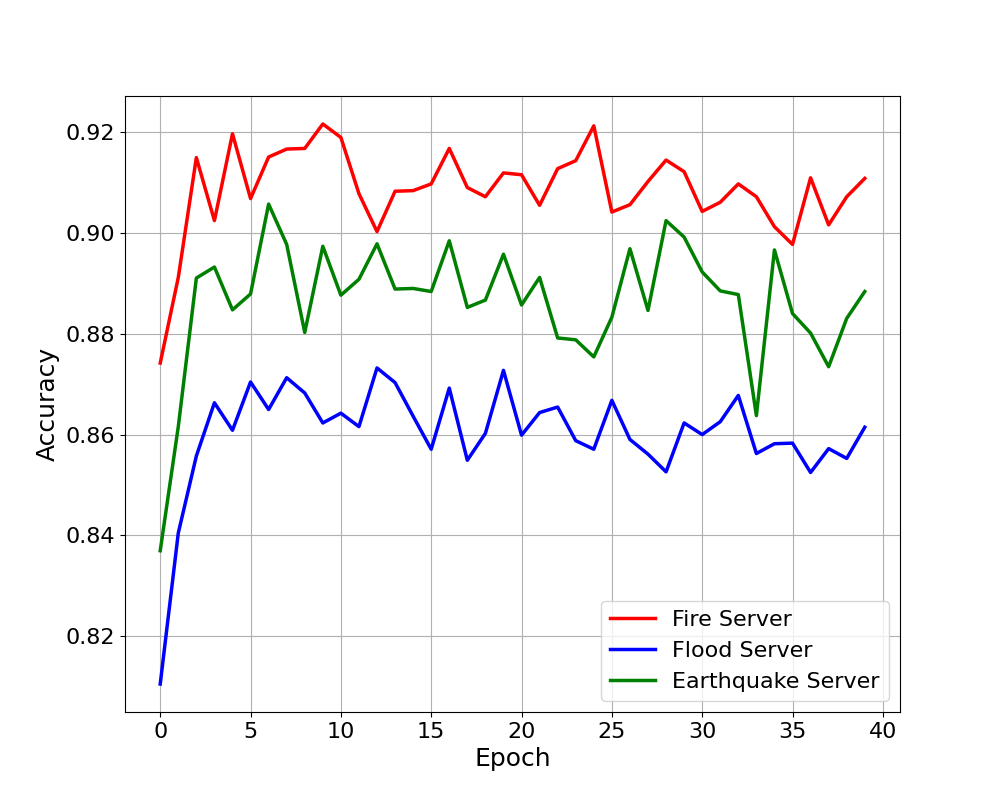
\includegraphics[width=\textwidth]{figures/chapter4/Server_Accuracies.png}
    \caption{Ακρίβεια Εξυπηρετητών στην Μετανοητική Μάθηση}
    \label{fig17}
\end{figure}

\begin{figure}[ht]
    \centering
    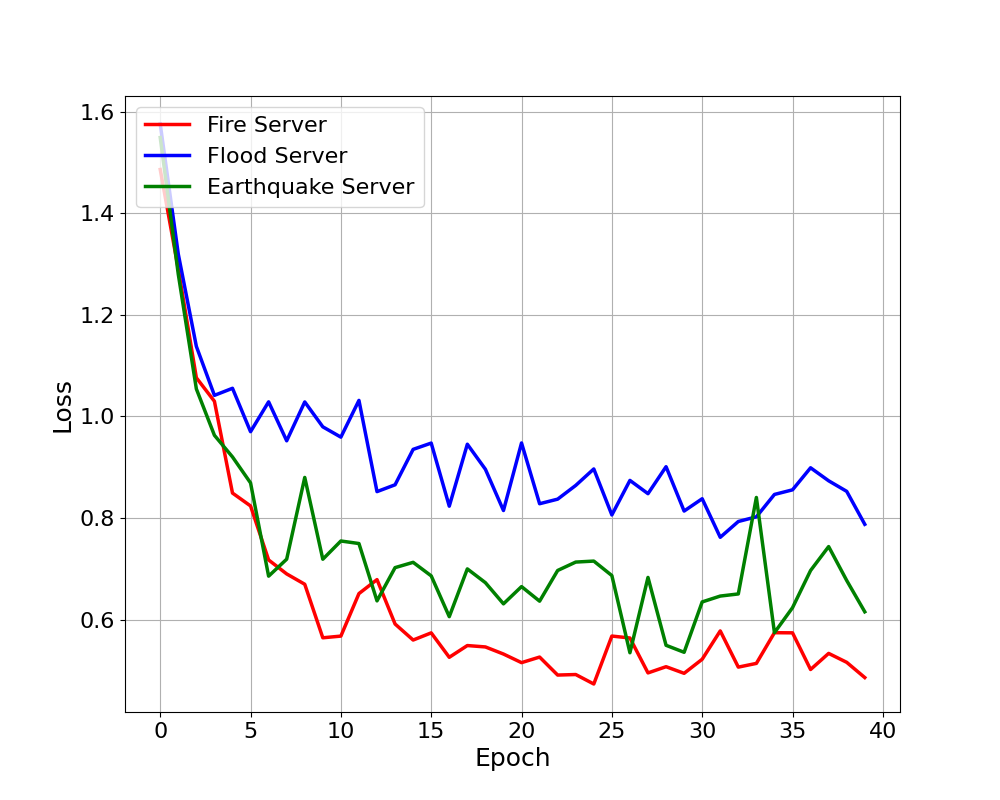
\includegraphics[width=\textwidth]{figures/chapter4/Server_Losses.png}
    \caption{Απώλεια Εξυπηρετητών στην Μετανοητική Μάθηση}
    \label{fig18}
\end{figure}

Όπως βλέπουμε στα σχήματα \ref{fig17}, \ref{fig18}, παρατηρούμε παρόμοια συμπεριφορά με τις προηγούμενες τεχνικές αντιστοίχισης. Όπως και σε προηγούμενες περιπτώσεις, έχουμε $Datasize_{fire} > Datasize_{flood} >Datasize_{earthquake}$, και επιπλέον ο εντοπισμός της φωτιάς είναι ένα πιο εύκολο πρόβλημα από ότι μιας πλημμύρας, αφού σε πλημμύρες έχουμε πιο ουδέτερα χρώματα, ενώ σε φωτιές πιο έντονα χρώματα και μεγάλες αλλαγές φωτεινότητας και σε σεισμούς πιο γήινα και ξηρά χρώματα. Επιπλέον, πολλές από τις ουδέτερες φωτογραφίες είναι πιο κοντά σε φωτογραφίες από πλημμύρες από ότι σε σεισμούς ή φωτιές, με αποτέλεσμα η διάκριση των δύο άλλων καταστροφών να είναι πιο απλή. Συνεπώς, για αυτούς τους λόγους, όπως και σε προηγούμενες περιπτώσεις έχουμε την καλύτερη απόδοση στον εξυπηρετητή που ανιχνεύει φωτιές, έπειτα στον εξυπηρετητή που ανιχνεύει σεισμούς και τέλος στον εξυπηρετητή που ανιχνεύει πλημμύρες παρότι $Datasize_{flood} >Datasize_{earthquake}$. 

Αντίστοιχα, για τις επιδόσεις των κόμβων, είναι εμφανές στα διαγράμματα \ref*{fig19} και \ref*{fig20}, πως έχουμε παρόμοια συμπεριφορά, μόνο που η ακρίβεια των κόμβων του εξυπηρετητή που ανιχνεύει για σεισμούς είναι μεγαλύτερη. Αυτό μας δείχνει πως παρότι οι κόμβοι τοπικά πετυχαίνουν καλύτερα αποτελέσματα, ο εξυπηρετητής δυσκολεύεται να γενικεύσει από τα βάρη που λαμβάνει από τους κόμβους του. Παρ' όλα ταύτα, είναι σημαντικό όμως να αναφέρουμε πως οι κόμβοι και οι εξυπηρετητές φαίνεται να μαθαίνουν αποτελεσματικά τις ιδιότητες των εικόνων, με αποτέλεσμα να πετυχαίνουν αρκετά υψηλές τελικές ακρίβειες. 

\newpage

\begin{figure}[H]
    \centering
    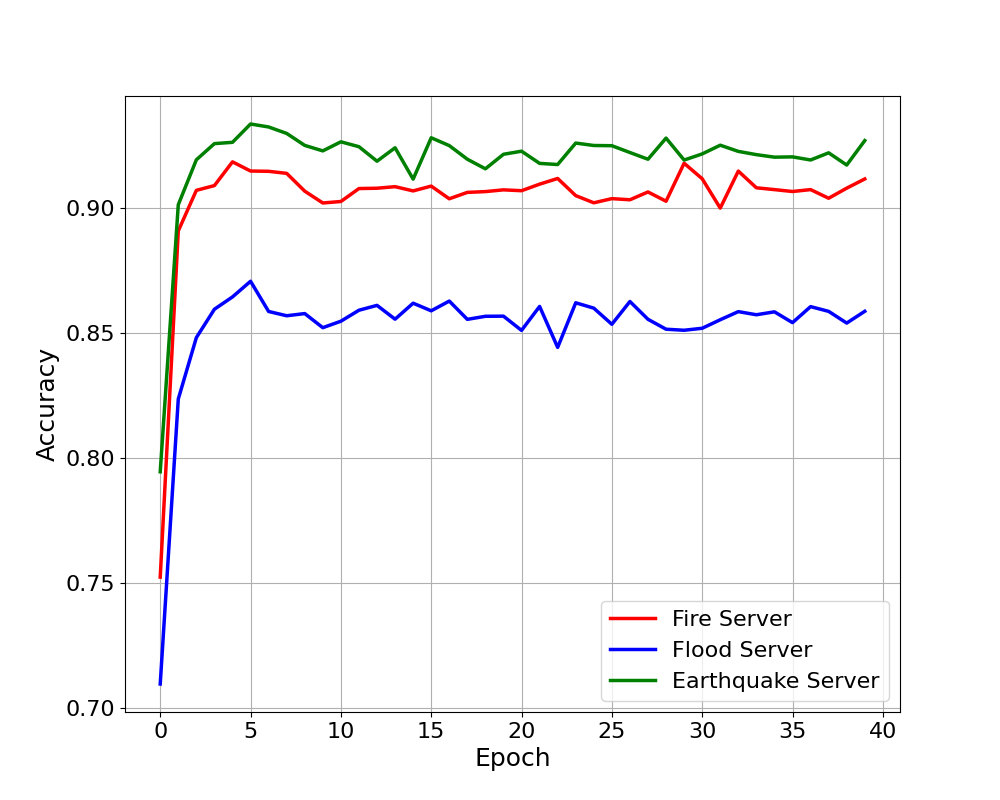
\includegraphics[width=0.85\textwidth]{figures/chapter4/User_Accuracies.png}
    \caption{Ακρίβεια κόμβων στην Μετανοητική Μάθηση}
    \label{fig19}
\end{figure}

\begin{figure}[H]
    \centering
    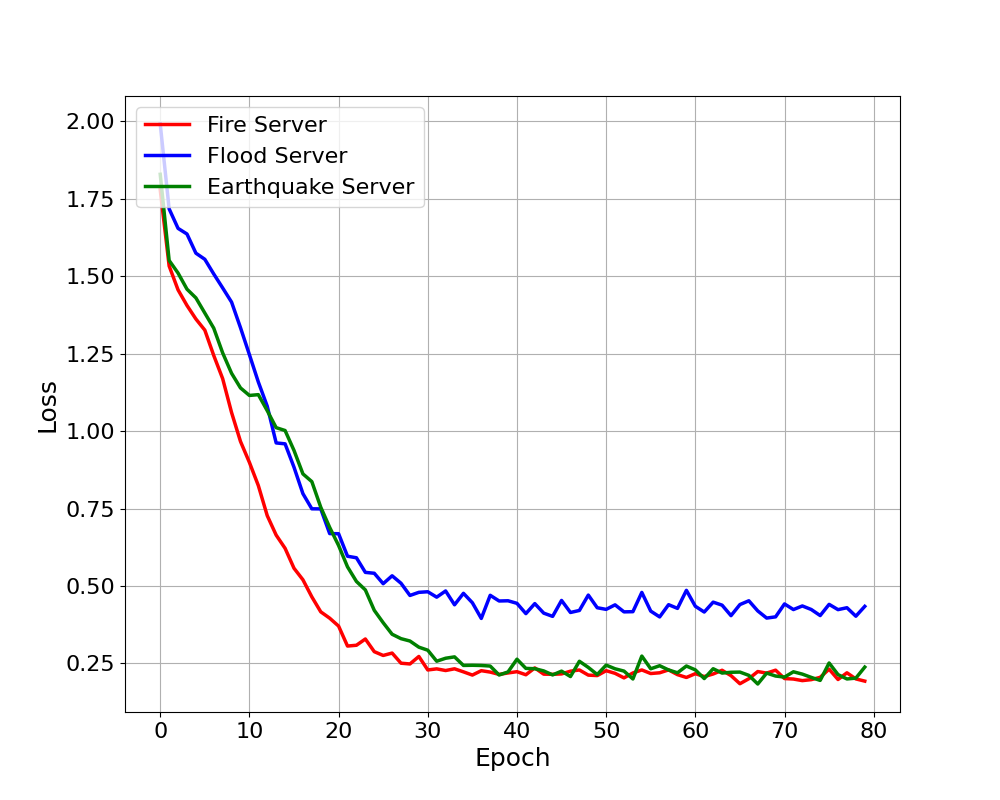
\includegraphics[width=0.85\textwidth]{figures/chapter4/User_Losses.png}
    \caption{Απώλεια κόμβων στην Μετανοητική Μάθηση}
    \label{fig20}
\end{figure}

\newpage

Όσον αφορά τις διαφορές μεταξύ των δύο αλγορίθμων Μετανοητικής Μάθησης, αλλά και όσον αφορά τις διαφορετικές περιοχές (Αστική Περιοχή, Προαστιακή Περιοχή, Αγροτική Περιοχή) παρατηρούμε τις εξής διαφορές:

\begin{figure}[H]
    \centering
    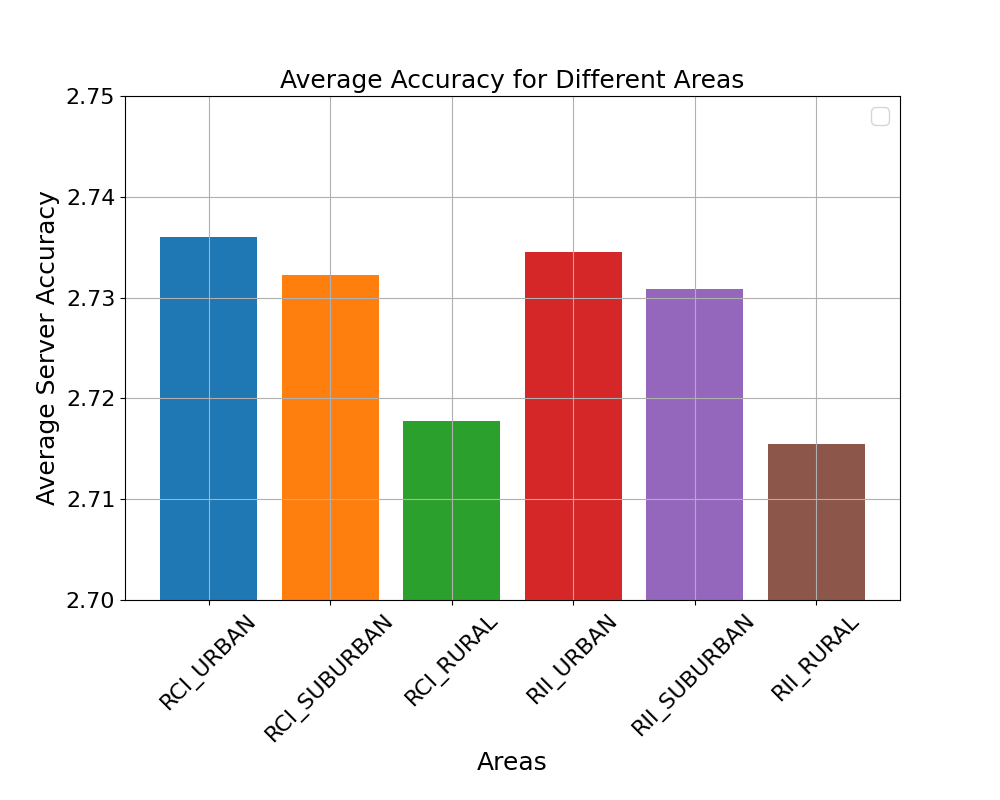
\includegraphics[width=0.75\textwidth]{figures/chapter4/Area_Average_Accuracy.png}
    \caption{Ακρίβεια Εξυπηρετητών Μετανοητικής Μάθησης σε διαφορετικές περιοχές}
    \label{fig21}
\end{figure}

\begin{figure}[H]
    \centering
    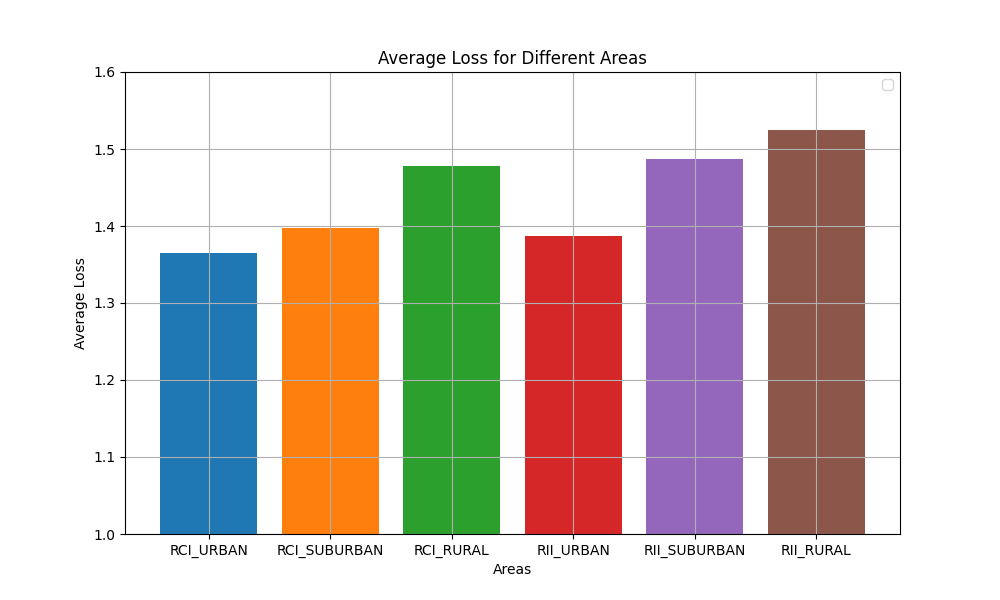
\includegraphics[width=0.75\textwidth]{figures/chapter4/Area_of_Average_Loss.png}
    \caption{Απώλεια Εξυπηρετητών Μετανοητικής Μάθησης σε διαφορετικές περιοχές}
    \label{fig22}
\end{figure}

\newpage

Όπως βλέπουμε στα παραπάνω σχήματα \ref{fig21} και \ref{fig22} υπάρχουν διαφοροποιήσεις στις επιδόσεις της Ομοσπονδιακής Μάθησης ανάλογα με τον αλγόριθμο που χρησιμοποιείται για την αντιστοίχιση και διαμόρφωση των κόμβων, αλλά και ανάλογα με την περιοχή στην οποία βρισκόμαστε. Έτσι, για τον αλγόριθμο Πλήρους Πληροφορίας, όπου βρίσκονται κατά βάση οι βέλτιστες λύσεις, παρατηρούμε πως πετυχαίνουμε την μικρότερη απώλεια στην Αστική Περιοχή, έπειτα στα Προάστια και τέλος στην Αγροτική Περιοχή, όπως είναι και το αναμενόμενο. Από την άλλη πλευρά, στον αλγόριθμο Ελλιπούς Πληροφορίας βλέπουμε μια απόκλιση στην Αστική Περιοχή που δεν συμβαδίζει με το προηγούμενο συμπέρασμα. Στον αλγόριθμο αυτό όμως δεν βρίσκουμε πάντα τις βέλτιστες λύσεις, λόγω απώλειας πλήρους πληροφορίας, και άρα οι τελικές αποφάσεις των κόμβων μπορεί να διαθέτουν λιγότερα δεδομένα στην Ομοσπονδιακή Μάθηση από ότι στην βέλτιστη λύση της Πλήρους Πληροφορίας. Όμως μένει πολύ κοντά στις επιδόσεις του αλγορίθμου Πλήρους Πληροφορίας.

\newpage

\section{Σύγκριση Μετανοητικής Μάθησης με Θεωρία Παιγνίων}

Επίσης, σημαντική πληροφορία παίρνουμε συγκρίνοντας τους δύο αλγορίθμους Μετανοητικής Μάθησης μεταξύ τους, αλλά και με τον αλγόριθμο του κεφαλαίου 2. Στο σημείο αυτό θα δούμε τα πλεονεκτήματα και μειονεκτήματα του κάθε αλγορίθμου και την επίδοσή του σε διαφορετικές περιπτώσεις. Όσον αφορά τα φυσικά μεγέθη τα οποία μελετάμε για τους κόμβους μας παρατηρούμε τα εξής:

\begin{figure}[H]
    \centering
    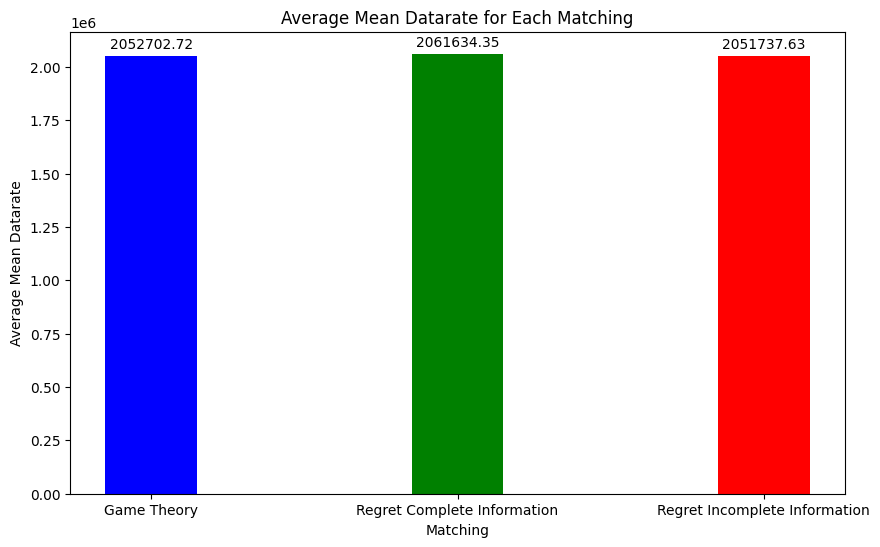
\includegraphics[width=0.85\textwidth]{figures/chapter4/Average_Mean_Datarate.png}
    \caption{Μέση ροή δεδομένων για τους κόμβους ανά αλγόριθμο αντιστοίχισης}
    \label{fig23}
\end{figure}

\begin{figure}[H]
    \centering
    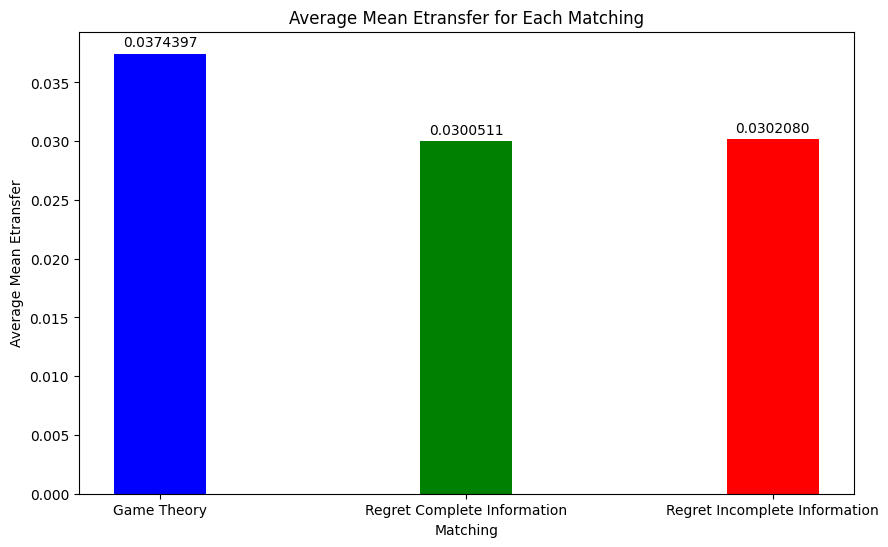
\includegraphics[width=0.85\textwidth]{figures/chapter4/Average_Mean_Etransfer.png}
    \caption{Μέση ενέργεια μετάδοσης για τους κόμβους ανά αλγόριθμο αντιστοίχισης}
    \label{fig24}
\end{figure}

\newpage

\begin{figure}[H]
    \centering
    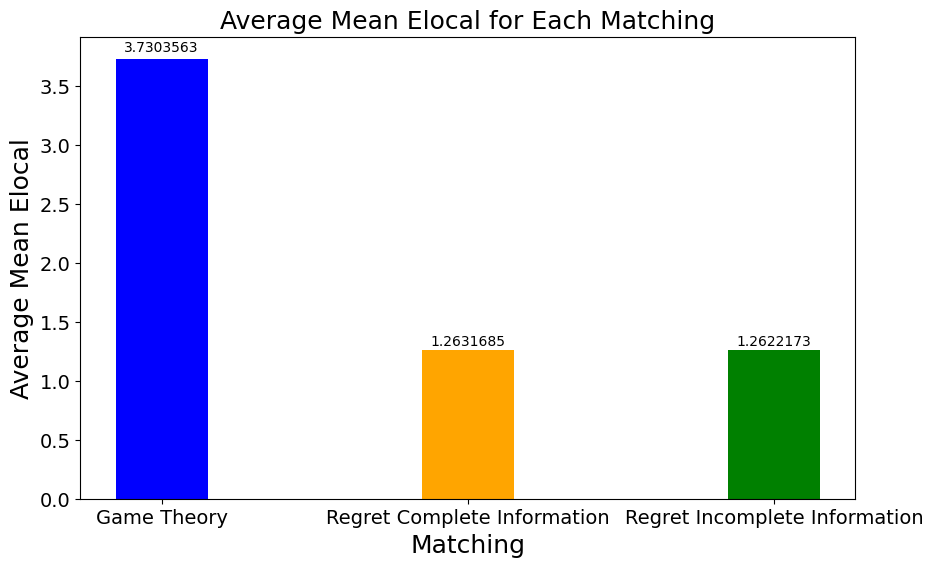
\includegraphics[width=0.85\textwidth]{figures/chapter4/Average_Mean_Elocal.png}
    \caption{Μέση ενέργεια εκπαίδευσης για τους κόμβους ανά αλγόριθμο αντιστοίχισης}
    \label{fig25}
\end{figure}

\begin{figure}[H]
    \centering
    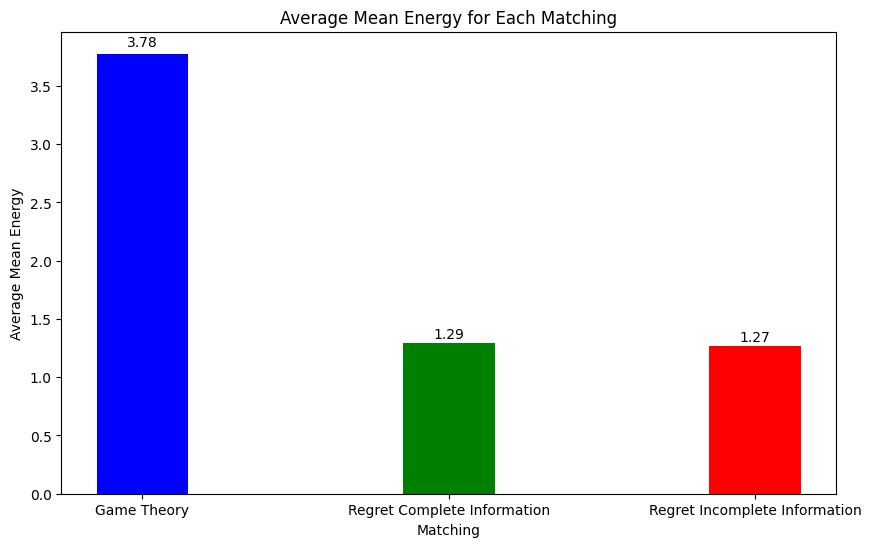
\includegraphics[width=0.85\textwidth]{figures/chapter4/Average_Mean_Energy.png}
    \caption{Μέση συνολική ενέργεια για τους κόμβους ανά αλγόριθμο αντιστοίχισης}
    \label{fig26}
\end{figure}

Αρχικά, όπως βλέπουμε στα παραπάνω διαγράμματα (\ref{fig23}, \ref{fig24}, \ref{fig25}, \ref{fig26}) οι αλγόριθμοι Μετανοητικής Μάθησης μας δίνουν πολύ καλύτερα αποτελέσματα, ειδικά σε εξοικονόμηση ενέργειας (είτε μετάδοσης, είτε εκπαίδευσης), πετυχαίνοντας παράλληλα καλύτερη μέση ροή μετάδοσης δεδομένων. Αυτό είναι λογικό, αφού οι δύο αλγόριθμοι δίνουν την δυνατότητα στους κόμβους να μεταβάλλουν τους πόρους που διαθέτουν στο σύστημά μας. Έτσι κάποιος πιο απομακρυσμένος κόμβος δεν "αναγκάζεται" να χρησιμοποιήσει όλους τους πόρους του καταναλώνοντας παραπάνω ενέργεια για μικρό κέρδος, ενώ αντίστοιχα σε ανταγωνιστικά μεγέθη όπως η Ροή Δεδομένων, ελευθερώνονται πόροι του συστήματος για τους πιο ενεργούς - σημαντικούς κόμβους. Από τους δύο αλγορίθμους Μετανοητικής Μάθησης, καλύτερα αποτελέσματα μας δίνει προφανώς ο αλγόριθμος Πλήρους Πληροφορίας, ο οποίος εξετάζει αναλυτικά την συμπεριφορά όλων των πιθανών ενεργειών του κάθε κόμβου παίρνοντας υπόψη και τις ενέργειες των υπολοίπων. Αυτό μπορεί να μην είναι προφανές για την ώρα, αφού όπως βλέπουμε στα διαγράμματα \ref{fig19} και \ref{fig20}, ο αλγόριθμος Ελλιπούς Πληροφορίας πετυχαίνει χαμηλότερη κατανάλωση ενέργειας από ότι ο Πλήρους Πληροφορίας.

\begin{figure}[H]
    \centering
    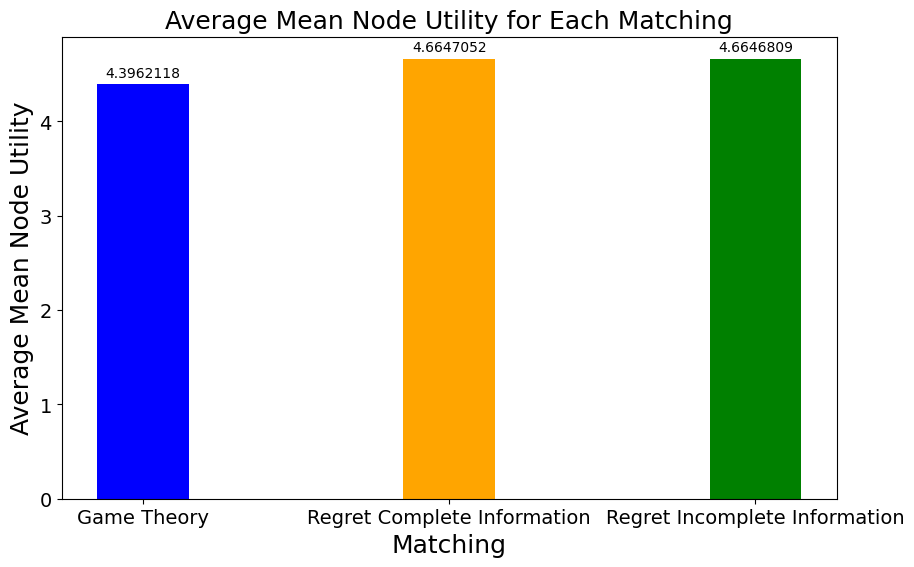
\includegraphics[width=0.85\textwidth]{figures/chapter4/Average_Mean_User_Utility.png}
    \caption{Μέση χρησιμότητα κόμβων ανά αλγόριθμο αντιστοίχισης}
    \label{fig27}
\end{figure}

\begin{figure}[H]
    \centering
    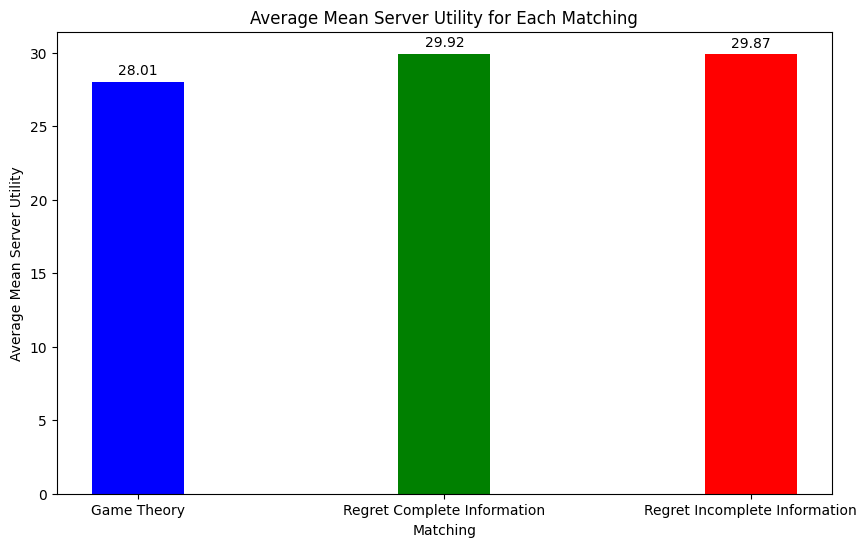
\includegraphics[width=0.85\textwidth]{figures/chapter4/Average_Mean_Server_Utility.png}
    \caption{Μέση χρησιμότητα εξυπηρετητών ανά αλγόριθμο αντιστοίχισης}
    \label{fig28}
\end{figure}

Έτσι, στα διαγράμματα \ref{fig27} και \ref{fig28}, όπου απεικονίζεται η μέση χρησιμότητα που επιτυγχάνουν οι κόμβους και οι εξυπηρετητές, γίνεται εμφανές πως ο αλγόριθμος Πλήρους Πληροφορίας πετυχαίνει καλύτερα αποτελέσματα από τον αλγόριθμο Ελλιπούς Πληροφορίας, αφού εν τέλει η μετρική με την οποία παίρνονται οι αποφάσεις στον εκάστοτε αλγόριθμο είναι η χρησιμότητα. Όμως και πάλι η διαφορά τους είναι πολύ μικρή. Αντίστοιχα και οι δύο αλγόριθμοι Μετανοητικής Μάθησης έχουν καλύτερες επιδόσεις από τον αλγόριθμο Θεωρίας Παιγνίων. 

Παρ' όλα ταύτα, ο αλγόριθμος Πλήρους Πληροφορίας έχει και κάποια μειονεκτήματα, συγκεκριμένα στον χρόνο που απαιτεί για να επιτύχει σύγκλιση. Πιο αναλυτικά βλέπουμε:

\begin{figure}[H]
    \centering
    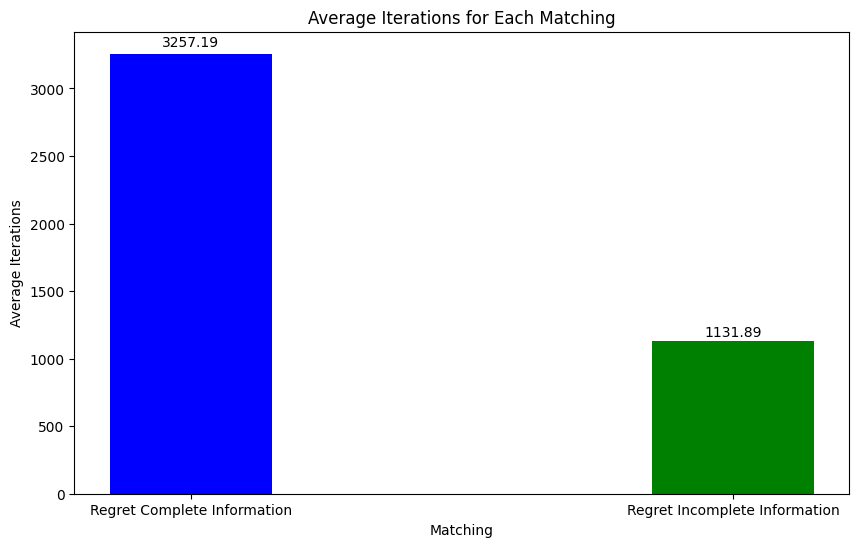
\includegraphics[width=0.85\textwidth]{figures/chapter4/Average_Iterations.png}
    \caption{Μέσος αριθμός επαναλήψεων ανά αλγόριθμο αντιστοίχισης}
    \label{fig29}
\end{figure}

\begin{figure}[H]
    \centering
    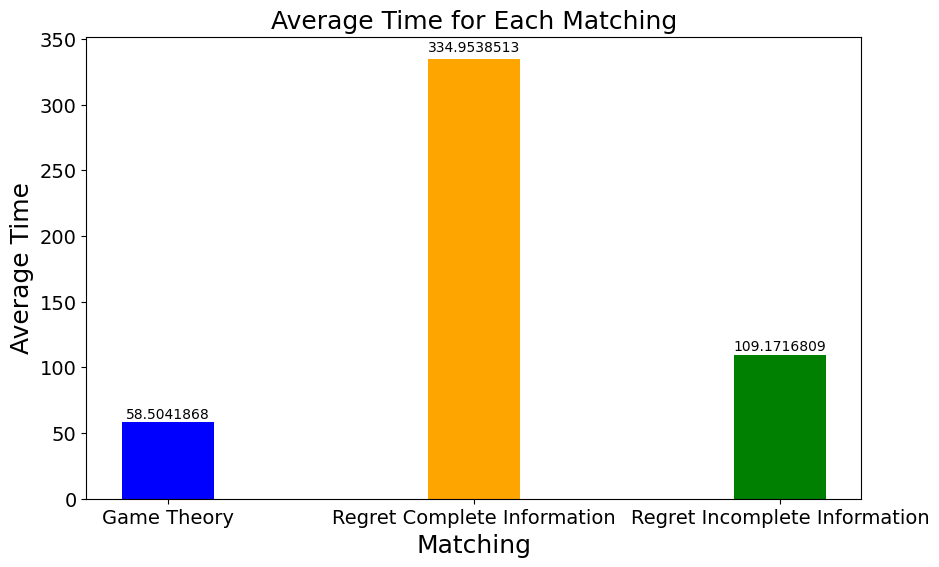
\includegraphics[width=0.85\textwidth]{figures/chapter4/Average_Time.png}
    \caption{Μέσος χρόνος εκτέλεσης ανά αλγόριθμο αντιστοίχισης}
    \label{fig30}
\end{figure}

Άρα παρότι εν γένει παίρνουμε καλύτερα αποτελέσματα με τον αλγόριθμο Πλήρους Πληροφορίας, έχει ένα μεγάλο μειονέκτημα όσον αφορά τον μεγάλο χρόνο που απαιτεί για την εκτέλεσή του (\ref{fig30}). Αυτό θα μπορούσε να είναι ένα κρίσιμο σημείο για συχνά μεταβαλλόμενα συστήματα, στα οποία απαιτείται συχνή επαναπροσαρμογή των παικτών. Παρότι, έχουμε μεγαλύτερο αριθμό επαναλήψεων στον αλγόριθμο Ελλιπούς Πληροφορίας (\ref{fig29}), κάθε επανάληψη του αλγορίθμου Πλήρους Πληροφορίας είναι πολύ πιο ακριβή υπολογιστικά, αφού πρέπει να εξετάσει τις πιθανές ενέργειες κάθε κόμβου στο σύστημα. Ειδικά για μεγαλύτερα σύνολα κόμβων η αντιστοίχιση γίνεται πάρα πολύ αργή.

\begin{figure}[ht]
    \centering
    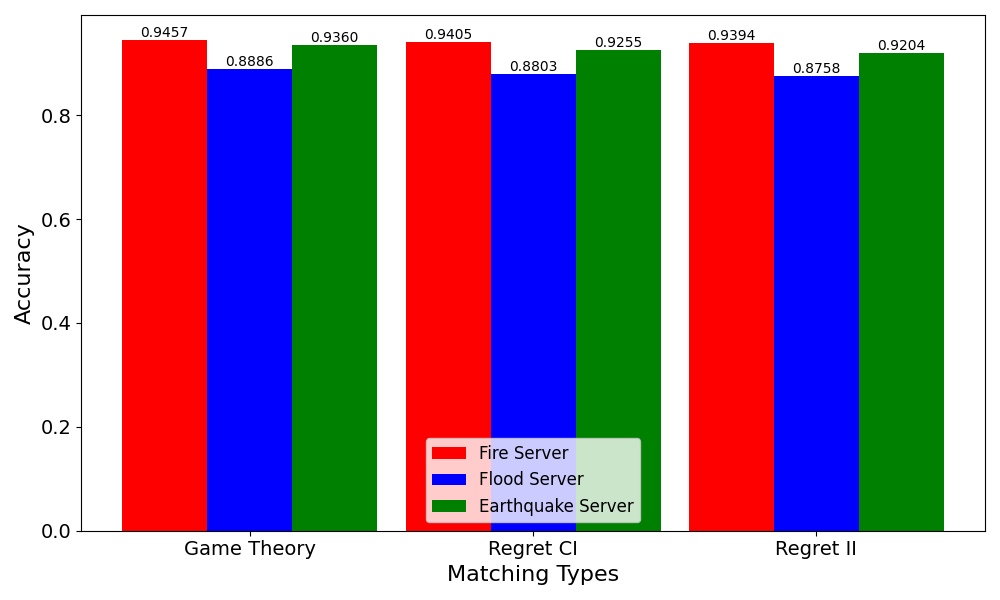
\includegraphics[width=0.85\textwidth]{figures/chapter4/accuracy_plot.png}
    \caption{Ακρίβεια Εξυπηρετητών ανά αλγόριθμο αντιστοίχισης}
    \label{fig31}
\end{figure}

\begin{figure}[ht]
    \centering
    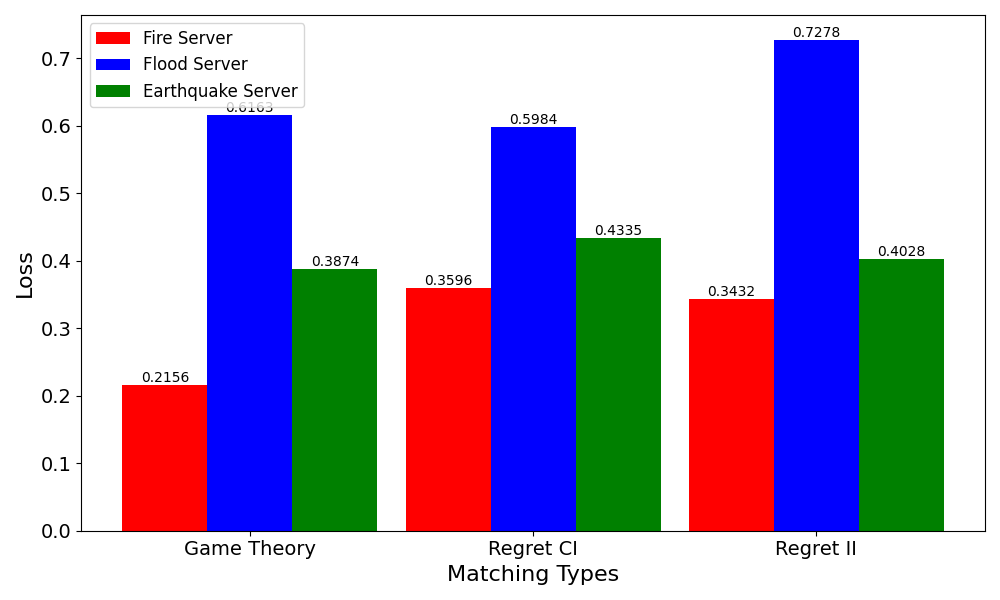
\includegraphics[width=0.85\textwidth]{figures/chapter4/loss_plot.png}
    \caption{Απώλεια Εξυπηρετητών ανά αλγόριθμο αντιστοίχισης}
    \label{fig32}
\end{figure}

\newpage

Στο κομμάτι της Ομοσπονδιακής Μάθησης παρατηρούμε πως ανάλογα με την σημασία κάθε κόμβου και τις απολαβές που μπορεί να συλλέξει, στους αλγορίθμους Μετανοητικής Μάθησης, ο κόμβος μπορεί να επιλέξει να διαθέσει λιγότερα δεδομένα στην διαδικασία της εκμάθησης. Αυτό έχει ως αποτέλεσμα, όπως φαίνεται στα \ref{fig31} και \ref{fig32}, να πετυχαίνουμε χειρότερα αποτελέσματα στην εκπαίδευση των μοντέλων με τους δύο αυτούς αλγορίθμους. Από την άλλη πλευρά, βλέπουμε πως και οι δύο αλγόριθμοι Μετανοητικής Μάθησης φτάνουν αρκετά κοντά σε επιδόσεις συγκριτικά με τον αλγόριθμο Θεωρίας Παιγνίων. Δεδομένου ότι πετυχαίνουμε αυτό το αποτέλεσμα, με τα μικρότερα σύνολα δεδομένων που χρησιμοποιούν οι αλγόριθμοι Μετανοητικής Μάθησης, είναι εμφανές πως το μοντέλο μας σε συνδυασμό με μια ορθή αντιστοίχιση και διαμόρφωση των κόμβων πετυχαίνει πολύ καλές επιδόσεις.

Αντίστοιχα, είναι σημαντικό να μελετήσουμε και την συμπεριφορά των αλγορίθμων μας ανάλογα με το πλήθος των κόμβων που καλούνται να διαχειριστούν.

\begin{figure}[ht]
    \centering
    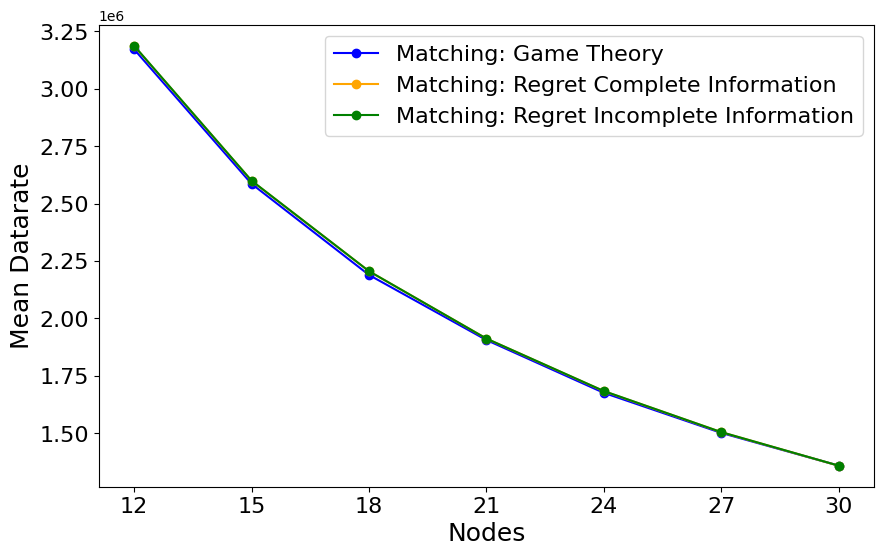
\includegraphics[width=\textwidth]{figures/chapter4/Mean_Datarate_vs_Users.png}
    \caption{Μέση ροή δεδομένων ανά αριθμό κόμβων ανά αλγόριθμο αντιστοίχισης}
    \label{fig33}
\end{figure}

Αρχικά, όπως είδαμε και παραπάνω, επαναλαμβάνεται η επικράτηση των αλγορίθμων Μετανοητικής Μάθησης σε σχέση με τον αλγόριθμο Θεωρίας Παιγνίων, λόγω της δυνατότητάς που τους έχουμε δώσει να διαμορφώνουν τη συμπεριφορά του κάθε κόμβου (\ref{fig33}, \ref{fig34}, \ref{fig35}, \ref{fig36}). Βλέπουμε πως η μέση ροή δεδομένων μειώνεται όσο ο αριθμός των κόμβων αυξάνεται (\ref{fig33}), το οποίο είναι λογικό, αφού οι κόμβοι μας μοιράζονται το κοινό εύρος ζώνης που διαθέτει ο εξυπηρετητής για την επικοινωνία με αυτούς. Όλοι οι αλγόριθμοι διατηρούν περίπου όμοια κλιμάκωση ανάλογα με τον αριθμό των κόμβων, με τον αλγόριθμο Πλήρους Πληροφορίας να πετυχαίνει το καλύτερο αποτέλεσμα, ακολουθούμενο από τον αλγόριθμο Ελλιπούς Πληροφορίας και τέλος από τον αλγόριθμο Θεωρίας Παιγνίων, όμως με ελάχιστες διαφορές (βλ \ref{fig23}). 

\begin{figure}[ht]
    \centering
    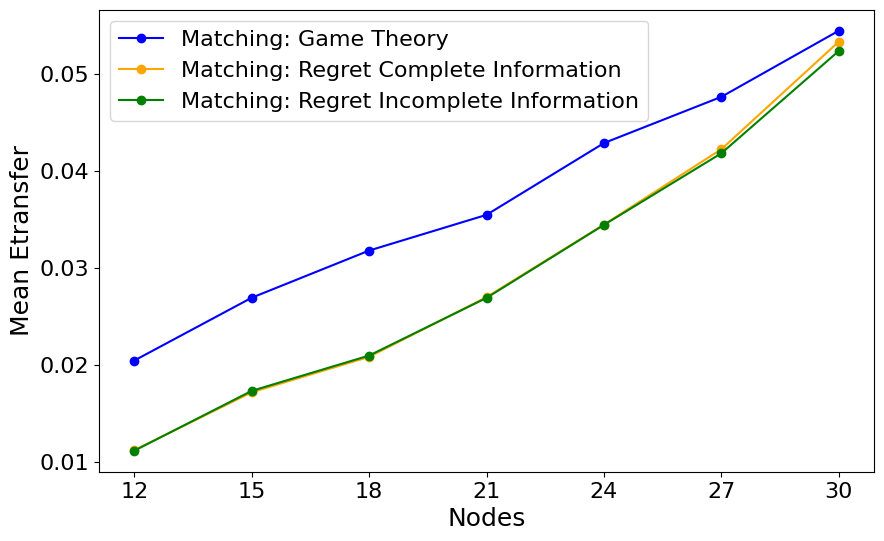
\includegraphics[width=\textwidth]{figures/chapter4/Mean_Etransfer_vs_Users.png}
    \caption{Μέση ενέργεια μετάδοσης ανά αριθμό κόμβων ανά αλγόριθμο αντιστοίχισης}
    \label{fig34}
\end{figure}

Και για τους τρεις αλγορίθμους η μέση ενέργεια μετάδοσης αυξάνεται όσο αυξάνεται και ο αριθμός των κόμβων (\ref{fig34}). Η συμπεριφορά αυτή είναι προϊόν του ανταγωνισμού, όπως είδαμε και στη ροή δεδομένων. Οι κόμβοι ανταγωνίζονται για πόρους και άρα προσπαθούν να διαθέσουν παραπάνω ισχύ, και άρα και ενέργεια, με σκοπό να διεκδικήσουν τους πόρους αυτούς. Συγκεκριμένα, όπως βλέπουμε και στο \ref{fig34} η ενέργεια μετάδοσης για τους αλγορίθμους Μετανοητικής Μάθησης αυξάνεται με μεγαλύτερο ρυθμό. Αυτό συμβαίνει επειδή όλοι οι κόμβους μεταδίδουν τον ίδιο αριθμό δεδομένων στον κεντρικό εξυπηρετητή, οι πιο απομακρυσμένοι, διεκδικώντας μικρότερο εύρος ζώνης θα απαιτούν περισσότερη ώρα για να μεταδώσουν την πληροφορία και άρα θα έχουν μεγαλύτερη κατανάλωση ενέργειας. Αξίζει να σημειώσουμε πως για 30 κόμβους ο αλγόριθμος Πλήρους Πληροφορίας φαίνεται να ωθεί τους κόμβους να διαθέσουν παραπάνω ισχύ και άρα μεγαλύτερη κατανάλωση ενέργειας για μετάδοση, απ' ότι ο αλγόριθμος Ελλιπούς Πληροφορίας.

Όπως βλέπουμε στο σχ.\ref{fig35}, καθώς ο αριθμός των κόμβων αυξάνεται, ο μέσος όρος της ενέργειας εκπαίδευσης σε κάθε περίπτωση μειώνεται. Αυτό συμβαίνει, διότι οι πιο απομακρυσμένοι κόμβοι έχουν στη διάθεσή τους μικρότερα σύνολα δεδομένων, αφού βρίσκονται πιο μακριά από τα κρίσιμα σημεία. Αντίστοιχα, επειδή οι αλγόριθμοι Μετανοητικής Μάθησης έχουν την δυνατότητα προσαρμογής του συνόλου δεδομένου που προσφέρει ο κάθε κόμβος στην Ομοσπονδιακή Μάθηση, επιτυγχάνουν πολύ μικρότερη μέση κατανάλωση ενέργειας εκπαίδευσης. 

\newpage

\begin{figure}[H]
    \centering
    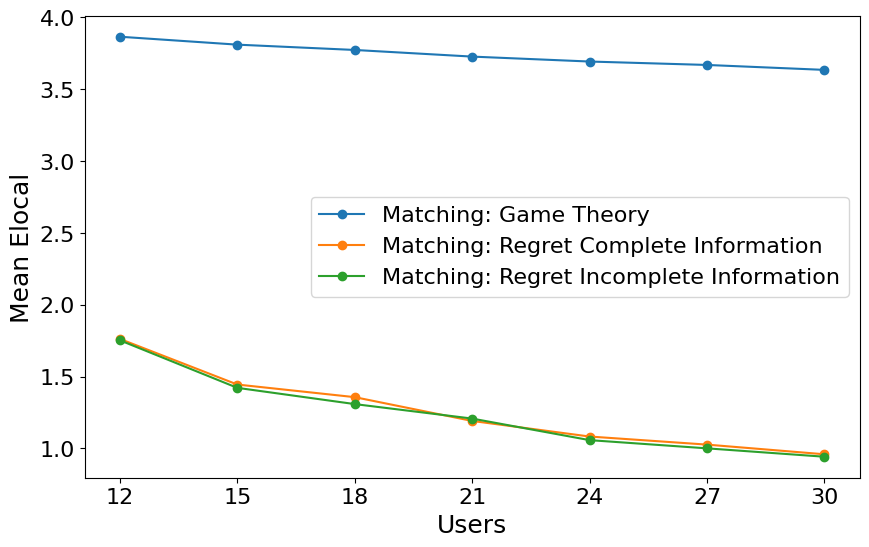
\includegraphics[width=\textwidth]{figures/chapter4/Mean_Elocal_vs_Users.png}
    \caption{Μέση ενέργεια εκπαίδευσης ανά αριθμό κόμβων ανά αλγόριθμο αντιστοίχισης}
    \label{fig35}
\end{figure}

\begin{figure}[H]
    \centering
    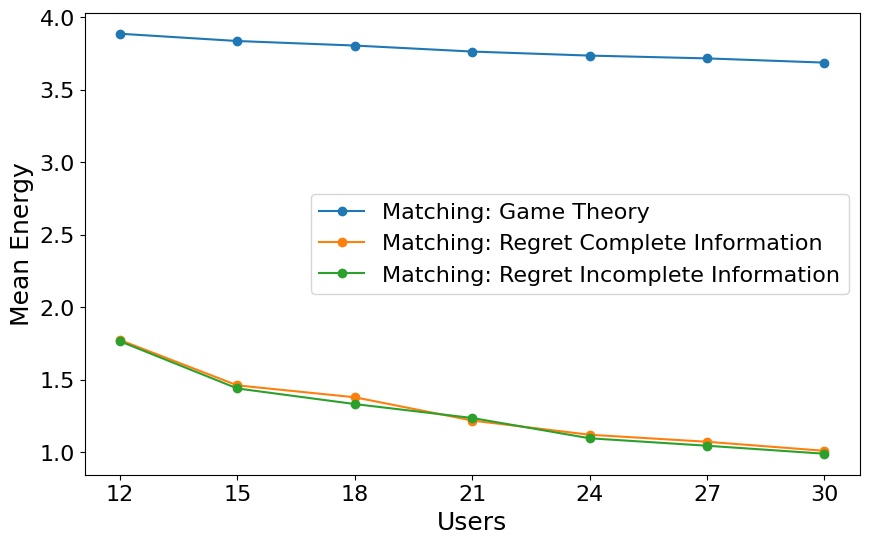
\includegraphics[width=\textwidth]{figures/chapter4/Mean_Energy_vs_Users.png}
    \caption{Μέση συνολική ενέργεια ανά αριθμό κόμβων ανά αλγόριθμο αντιστοίχισης}
    \label{fig36}
\end{figure}

\newpage

Για τον ίδιο λόγο επίσης η μέση κατανάλωση ενέργειας εκπαίδευσης μειώνεται με μεγαλύτερο ρυθμό στους αλγορίθμους Μετανοητικής Μάθησης. Στον αλγόριθμο Πλήρους Πληροφορίας βλέπουμε πως γενικά έχουμε μια μεγαλύτερη κατανάλωση ενέργειας, όπου όπως είδαμε και προηγουμένως οφείλεται στην καλύτερη αξιοποίηση των συνόλων δεδομένων των κόμβων. Αντίστοιχα, στο σχ.\ref{fig36} βλέπουμε πως η μέση συνολική ενέργεια παρουσιάζει αντίστοιχη μορφή με την μέση ενέργεια εκπαίδευσης, αφού το μεγαλύτερο μέρος της ενέργειας που καταναλώνεται αφορά την τοπική εκπαίδευση για κάθε κόμβο. Αξίζει να σημειωθεί πως μπορεί να παρατηρηθεί και η ανάποδη συμπεριφορά. Για παράδειγμα, ο αλγόριθμος Ελλιπούς Πληροφορίας μπορεί να δεσμεύσει παραπάνω δεδομένα (από το βέλτιστο) για κάθε κόμβο και άρα να είναι για αυτόν μεγαλύτερη η ενέργεια εκπαίδευσης. Αντίστοιχα σε τέτοιες περιπτώσεις είναι πιθανό να παρατηρηθούν και καλύτερες αποδόσεις στην εκπαίδευση των μοντέλων. Όμως πάντα ο αλγόριθμος Πλήρους Πληροφορίας πετυχαίνει σταθερά υψηλότερες χρησιμότητες, που αφορούν και την μετρική απόδοσης των αλγορίθμων μας, απ' ότι ο Ελλιπούς Πληροφορίας. 

\begin{figure}[H]
    \centering
    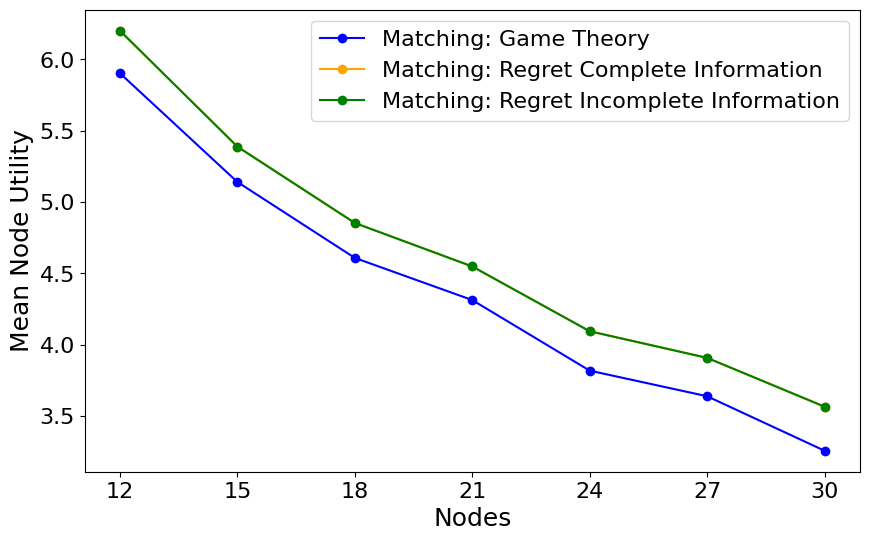
\includegraphics[width=\textwidth]{figures/chapter4/Mean_User_Utility_vs_Users.png}
    \caption{Μέση χρησιμότητα κόμβων ανά αριθμό κόμβων ανά αλγόριθμο αντιστοίχισης}
    \label{fig37}
\end{figure}

\newpage

\begin{figure}[H]
    \centering
    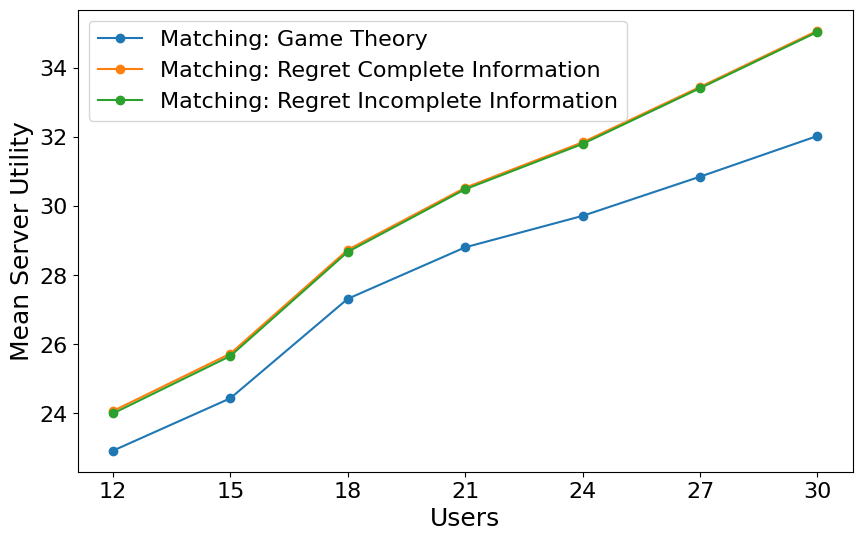
\includegraphics[width=\textwidth]{figures/chapter4/Mean_Server_Utility_vs_Users.png}
    \caption{Μέση χρησιμότητα εξυπηρετητών ανά αριθμό κόμβων ανά αλγόριθμο αντιστοίχισης}
    \label{fig38}
\end{figure}

Όπως βλέπουμε στο σχ.\ref{fig37} η μέση χρησιμότητα των κόμβων πέφτει όσο περισσότεροι κόμβοι ζουν στο σύστημά μας. Αυτό είναι λογικό, αφού με περισσότερους κόμβους έχουμε και μεγαλύτερο ανταγωνισμό για τους μοιραζόμενους πόρους, ενώ παράλληλα οι νέοι κόμβοι, όντας πιο μακρινοί από τα κρίσιμα σημεία, είναι μικρότερης σημασίας και άρα έχουν μικρότερες μέγιστες τιμές χρησιμότητας, ρίχνοντας το μέσο όρο. Αυτό φαίνεται αντίστοιχα στο σχ.\ref{fig38}, όπου όσο περισσότεροι κόμβοι είναι διαθέσιμοι, τόσο λιγότερο κλιμακώνει η χρησιμότητα των εξυπηρετητών. Επιπλέον, η χρησιμότητα των εξυπηρετητών αυξάνεται με την αύξηση των κόμβων, αφού περισσότεροι κόμβους είναι διαθέσιμοι σε κάθε εξυπηρετητή.

Όσον αφορά τον χρόνο εκτέλεσης και τον αριθμό επαναλήψεων που απαιτεί κάθε αλγόριθμος (σχ.\ref{fig39} και σχ.\ref{fig40}) μπορούμε να δούμε πως ο αλγόριθμος Πλήρους Πληροφορίας αυξάνει σε υπολογιστικό κόστος πολύ γρήγορα σε σχέση με τον αριθμό των κόμβων. Αντίθετα, ο Ελλιπούς Πληροφορίας παρουσιάζει ίδιο κόστος και σε επαναλήψεις και σε χρόνο, ανεξαιρέτως του πλήθους των κόμβων καθιστώντας τον μη ιδανικό για μικρά Ν, αλλά δίνοντάς του πολύ καλή κλιμάκωση.  Τέλος ο αλγόριθμος Θεωρίας Παιγνίων αυξάνει αργά σε υπολογιστικό κόστος, με γραμμικό τρόπο. Για τους δύο αλγορίθμους Μετανοητικής Μάθησης μπορούμε να παρατηρήσουμε επίσης το εξής. Ο αλγόριθμος Ελλιπούς Πληροφορίας φαίνεται να δυσκολεύεται στη σύγκλιση, πιθανότατα λόγω της ελλιπούς του πληροφορίας, αλλά το φθηνό υπολογιστικό του κόστος τον καθιστά πολύ γρήγορο στην εκτέλεση και άρα ιδανικό για οποιουδήποτε τύπου συστήματα. Αντίθετα φαίνεται ο αλγόριθμος Πλήρους Πληροφορίας να επηρεάζεται στην σύγκλιση και άρα και στον χρόνο εκτέλεσης από την θέση των εκάστοτε κόμβων. Όσο περισσότερους κόμβους διαθέτουμε και όσο αυτοί είναι πιο απομακρυσμένοι τόσο πιο πολλές επαναλήψεις φαίνεται να απαιτούνται για την σύγκλιση του αλγορίθμου και άρα μεγαλώνει ο χρόνος εκτέλεσης.

\newpage

\begin{figure}[H]
    \centering
    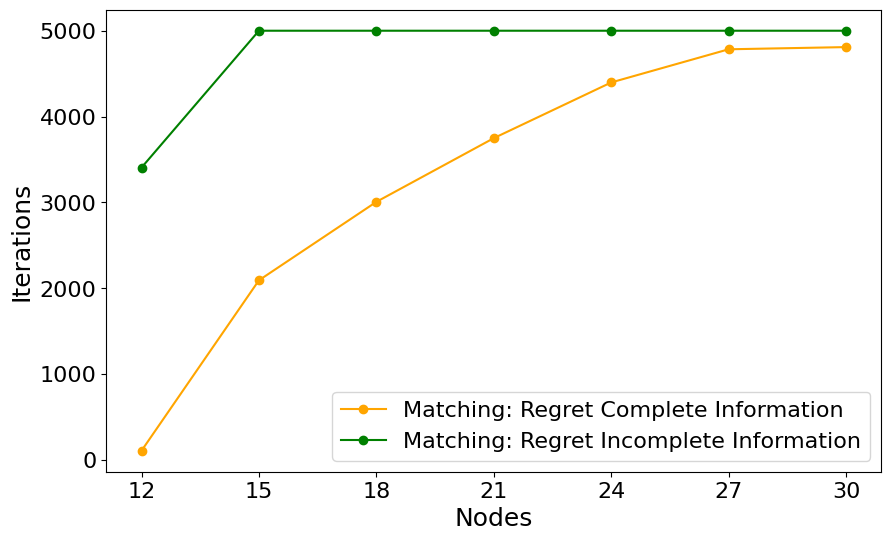
\includegraphics[width=\textwidth]{figures/chapter4/Iterations_vs_Users.png}
    \caption{Μέσος αριθμός επαναλήψεων ανά αριθμό κόμβων ανά αλγόριθμο αντιστοίχισης}
    \label{fig39}
\end{figure}

\begin{figure}[H]
    \centering
    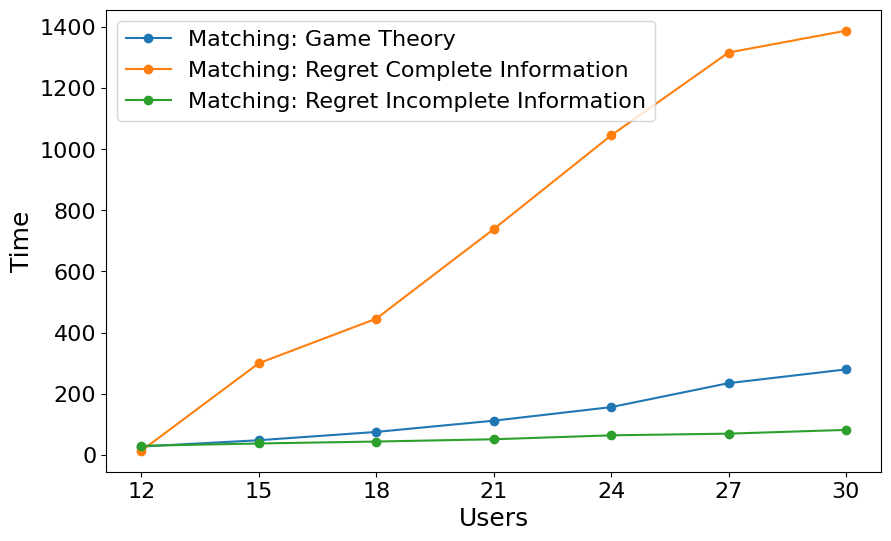
\includegraphics[width=\textwidth]{figures/chapter4/Time_vs_Users.png}
    \caption{Μέσος χρόνος εκτέλεσης ανά αριθμό κόμβων ανά αλγόριθμο αντιστοίχισης}
    \label{fig40}
\end{figure}

\newpage

Μελετώντας παραπάνω αυτή τη συμπεριφορά βλέπουμε:

\begin{figure}[H]
    \centering
    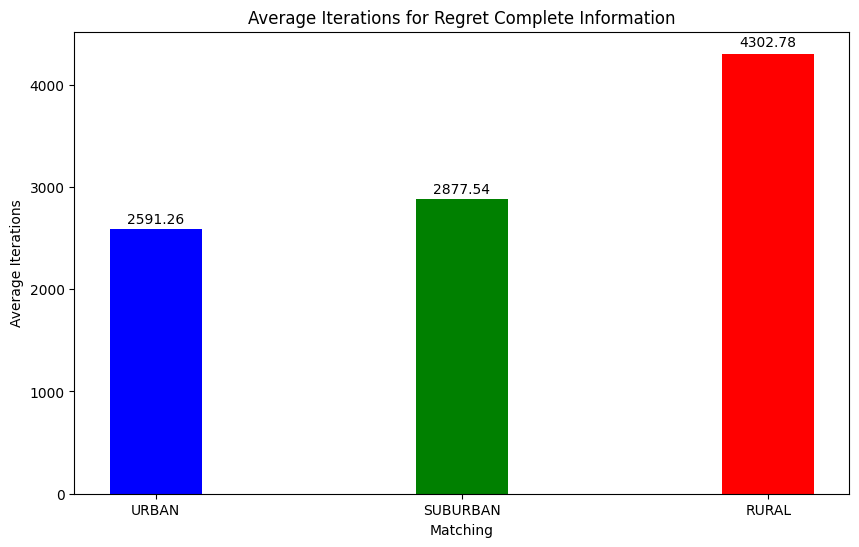
\includegraphics[width=\textwidth]{figures/chapter4/Average_Iterations_per_area_RCI.png}
    \caption{Επαναλήψεις Αλγορίθμου Πλήρους Πληροφορίας ανά Περιοχή}
    \label{fig41}
\end{figure}

\begin{figure}[H]
    \centering
    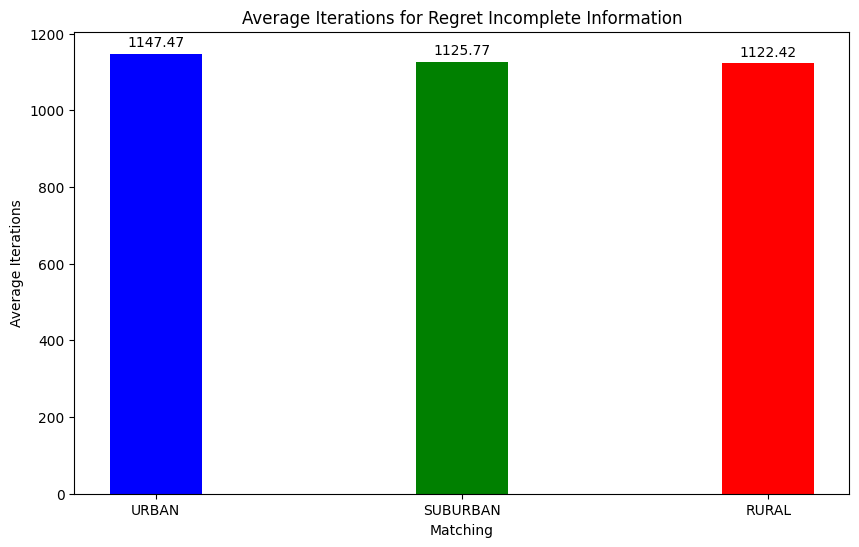
\includegraphics[width=\textwidth]{figures/chapter4/Average_Iterations_per_area_RII.png}
    \caption{Επαναλήψεις Αλγορίθμου Ελλιπούς Πληροφορίας ανά Περιοχή}
    \label{fig42}
\end{figure}

\newpage

\begin{figure}[H]
    \centering
    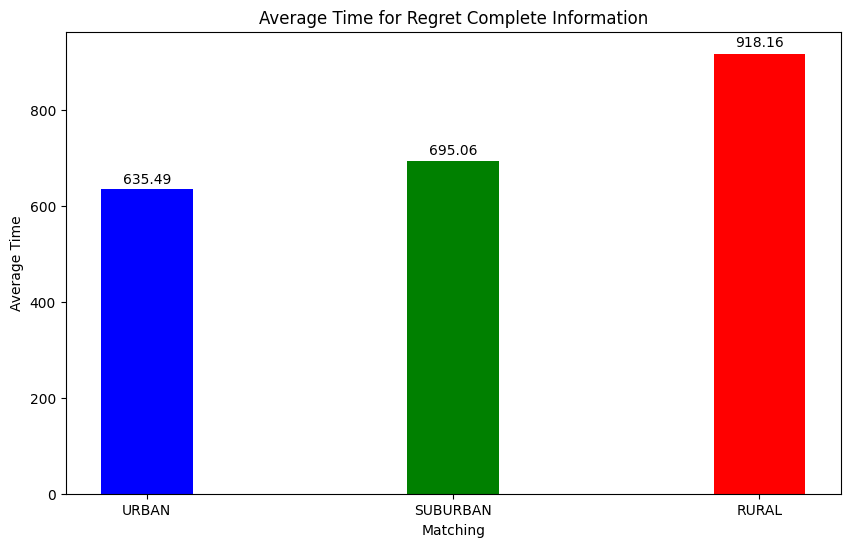
\includegraphics[width=\textwidth]{figures/chapter4/Average_Time_per_area_RCI.png}
    \caption{Χρόνος Εκτέλεσης Αλγορίθμου Πλήρους Πληροφορίας ανά Περιοχή}
    \label{fig43}
\end{figure}

\begin{figure}[H]
    \centering
    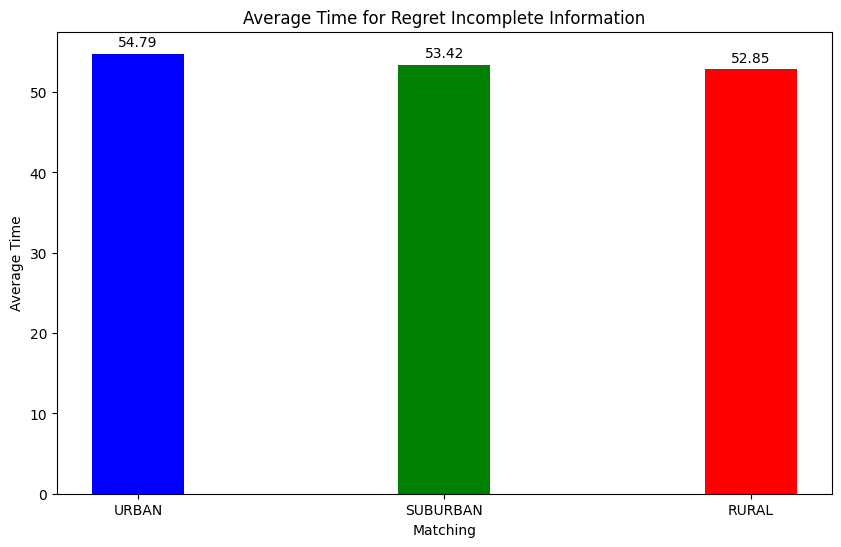
\includegraphics[width=\textwidth]{figures/chapter4/Average_Time_per_area_RII.png}
    \caption{Χρόνος Εκτέλεσης Αλγορίθμου Ελλιπούς Πληροφορίας ανά Περιοχή}
    \label{fig44}
\end{figure}

\newpage

Στα σχήματα \ref{fig41} και \ref{fig42} γίνεται εμφανής η παρατήρηση που κάναμε παραπάνω. Όσο πιο πολλοί απομακρυσμένοι κόμβοι ζουν στο σύστημά μας τόσο περισσότερο δυσκολεύεται να φτάσει σε σύγκλιση ο αλγόριθμος Πλήρους Πληροφορίας σε αντίθεση με τον Ελλιπούς Πληροφορίας. Αντίστοιχα αυτό μας οδηγεί στα διαγράμματα \ref{fig43} και \ref{fig44}, όπου αντίστοιχα με τον αριθμό των επαναλήψεων του αλγορίθμου έχουμε και διαμόρφωση των χρόνων εκτέλεσης. Η διαφοροποίηση αυτή στους δύο αλγορίθμους συμβαίνει, διότι όσο πιο μακρινούς κόμβους έχουμε, τόσο πιο δύσκολη είναι η σύγκλιση στον αλγόριθμο Πλήρους Πληροφορίας στην βέλτιστη διαμόρφωση του κόμβου, διότι αυτή κατά πάσα πιθανότητα διαφέρει από άλλες κατά πολύ λίγο και συνεπώς, οι τιμές μετάνοιας για τις κοντινές αυτές πράξεις μειώνονται με πολύ αργό ρυθμό. Αντίθετα, στον αλγόριθμο Ελλιπούς Πληροφορίας η αρχικοποίηση των χρησιμοτήτων, σε συνδυασμό με το γεγονός πως σε κάθε επανάληψη δεν ενημερώνονται όλες οι χρησιμότητες, αλλά και λόγω του λευκού θορύβου που δημιουργεί μεγαλύτερες διαφορές στις χρησιμότητες, επιτυγχάνουμε παρόμοια σύγκλιση σε όλες τις περιπτώσεις.

\begin{figure}[ht]
    \centering
    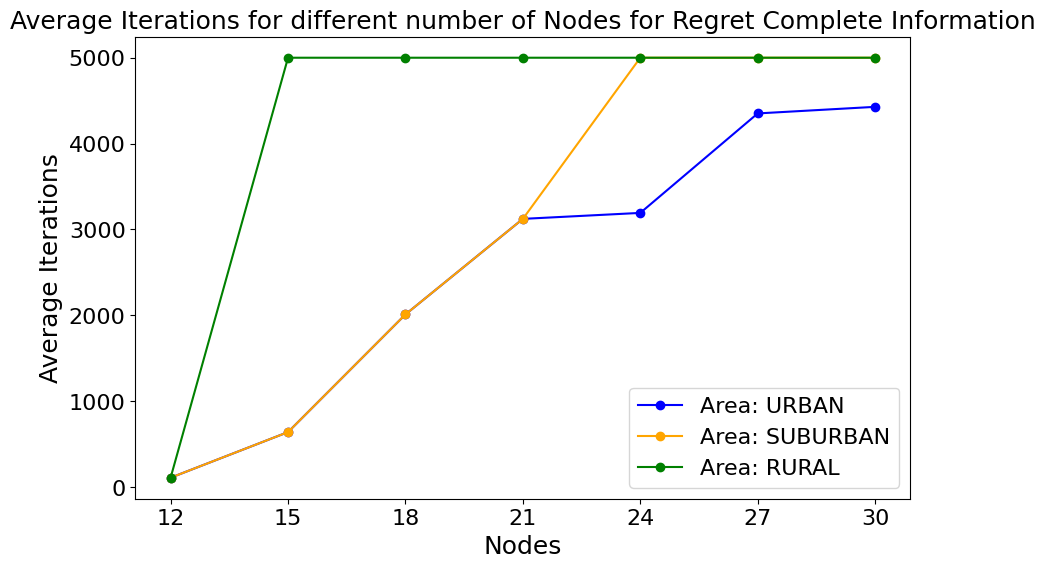
\includegraphics[width=\textwidth]{figures/chapter4/RCI_Iterations_vs_Users_per_Area.png}
    \caption{Μέσος αριθμός επαναλήψεων ανά αριθμό κόμβων ανά περιοχή για τον αλγόριθμο Πλήρους Πληροφορίας}
    \label{fig45}
\end{figure}

Στο διάγραμμα \ref{fig45} βλέπουμε πιο αναλυτικά την διακύμανση των απαιτούμενων επαναλήψεων για τον αλγόριθμο Πλήρους Πληροφορίας, ανά περιοχή, όσο αυξάνεται ο αριθμός των κόμβων. Είναι εμφανές, πως όταν αρχίσουν σε κάθε περιοχή να εισέρχονται πιο απομακρυσμένοι κόμβοι, η σύγκλιση δυσχεραίνει. Αντίστοιχα, όσο περισσότεροι κόμβοι υπάρχουν στο σύστημά μας, τόσο πιο δύσκολη γίνεται η σύγκλιση, αφού κατ' αρχήν θέλουμε όλοι μας οι κόμβοι να συγκλίνουν, ενώ επιπλέον, αφού το περιβάλλον μας είναι ανταγωνιστικό, οι αλλαγές συμπεριφοράς ενός κόμβου είναι πιθανό να επηρεάσουν και τους υπολοίπους στη βέλτιστη επιλογή τους.